\documentclass[12pt,a4paper,twoside]{article}
\usepackage[utf8]{inputenc}
\usepackage[spanish]{babel}
\usepackage{amsmath}
\usepackage{amsfonts}
\usepackage{amssymb} 
\usepackage{graphicx}

% Marca de agua

\usepackage{transparent}
\usepackage{eso-pic}
\usepackage{lipsum}

%\AddToShipoutPicture{
%\put (0,0){
%\parbox[b][\paperheight]{\paperwidth}{
%\vfill
%\centering
%{\transparent{0.2} 
\includegraphics[scale=0.8]{Imagenes/Geovalores.png}}
%\vfill
%}
%}
%}

% ----------------- Encabezado --------------------

\usepackage{geometry}
\newgeometry{bottom=4cm, top=3cm, left=3cm, right=3cm}

\usepackage{fancyhdr}
\pagestyle{fancy}

%\lhead{\transparent{0.3} 
\includegraphics[scale=0.18]{Imagenes/Geovalores.png}
%}	
\chead{ID 9302}
\rhead{
\includegraphics[scale=0.25]{Imagenes/QR.png} }


\cfoot{ \tiny Interventoría • Consultoría • Gestión Predial • Ambiental • Social • Avalúos • SIG  Cartografía • Catastro
	
	www.interval.co 
		
	Bogotá D.C Colombia
}

\renewcommand{\footrulewidth}{0.08pt}

\usepackage{multicol}
\author{}
\title{Informe de Avalúo}

\begin{document}
	

% ---------------------- Datos generales del inmueble --------------------

\newcommand{\Direccion}[1]{Calle 175 No. 20A -65}
\newcommand{\VeredaBarrio}[1]{Comuneros}
\newcommand{\Municipio}[1]{Bucaramanga}
\newcommand{\Departamento}[1]{Santander}
\newcommand{\Propietarios}[1]{COLOMBIA TELECOMUNICACIONES S.A E.S.P BIC}
\newcommand{\Matricula}[1]{300-17810}
\newcommand{\EscrituraAportada}[1]{Copia simple de la Escritura Publica No. 4126 del 26 de Noviembre de 1997, otorgada en la Notaria 2 de Bucaramanga.}
\newcommand{\DocAdquisicion}[1]{Copia simple de la Escritura Publica No. 4126 del 26 de Noviembre de 1997, otorgada en la Notaria 2 de Bucaramanga.}
\newcommand{\RPH}[1]{No aplica}
% Índice de contenido
\part*{AVALÚO COMERCIAL INMUEBLE URBANO}

\bigskip 
\bigskip 
\bigskip 
\bigskip 
\bigskip 
\bigskip 

\section*{DIRECCIÓN}

\subsection*{\Direccion}
\subsection*{\VeredaBarrio}
\subsection*{\Municipio}
\subsection*{\Departamento}

\bigskip 
\bigskip 
\bigskip 
\bigskip 
\bigskip 
\bigskip 

\section*{Solicitado Por}

\subsection*{\Propietarios}

\bigskip 
\bigskip 
\bigskip 
\bigskip 
\bigskip 
\bigskip 

\section*{DATOS DEL PERITO}

\subsection*{Juan Palma}
\subsection*{RAA. Aval-1013620663}

\bigskip 
\bigskip 
\bigskip 
\bigskip 
\bigskip 
\bigskip 

\section*{FECHA}

\subsection*{16 de Agosto del 2024}
	
% Marca de agua

% Índice de contenido

\clearpage

\tableofcontents

\clearpage


\section{Información básica}

\subsection{Identificación del cliente}

\begin{tabular}{ l p{7.5cm} }
	
	\textbf{Cliente:} & \Propietarios. \\
	\textbf{Documento de identificación:} & Nit. 830.122.566-1.\\
	\textbf{Destinatario del avalúo:} & \Propietarios. \\
	
\end{tabular}


\subsection{Objeto de la Valuación}

El presente estudio se realiza con el fin de conocer los factores físicos, económicos y jurídicos que inciden en el valor comercial del bien inmueble objeto de avalúo y establecer el valor de mercado mas probable, entendiendo este como ''la cuantiá estimada por la que un bien podría intercambiarse en la fecha de valuación, entre un comprador dispuesto a comprar y un vendedor dispuesto a vender, en una transacción libre tras una comercialización adecuada, en la que las partes hayan actuado con la información suficiente de manera prudente y sin coacción.''\footnote{Norma técnica sectorial 01}.

\subsection{Tipo de avalúo}

Comercial.

\subsection{Ubicación del inmueble}

\begin{description}
	
	\item[Tipo de inmueble: ] Lote de terreno junto con la construcción sobre el levantada.
	\item[Dirección: ] \Direccion.
	\item[Departamento: ] \Departamento.
	\item[Municipio: ] \Municipio.
%	\item[Barrio o Vereda: ] \VeredaBarrio.
	\item[Coordenadas: ] \textbf{Log:} 	
 -73.127821, \textbf{Lat:} 	
 7.137223. 
	%\item[Localidad:] 11-Suba.
	%\item[UPL:] 16-Bosa.
	%\item[Sector:] 009129-Villa Del Prado.
	
\end{description}
 
\subsection{Fecha de visita}
 
03 de Agosto del 2024.

\subsection{Fecha del informe}

16 de Agosto del 2024.

\subsection{Documentación aportada}

\begin{itemize}
\item Certificado de tradición y libertad según matricula inmobiliaria No. 300-17810, impreso el 31 de Julio del 2024, expedido por la oficinas de registro de instrumentos públicos de Bucaramanga.
%\item Certificado de tradición y libertad según matricula inmobiliaria No. 040-616295, impreso el 29 de Julio del 2021, expedido por la oficinas de registro de instrumentos públicos de Barranquilla.
\item Copia simple de la Escritura Publica No. 4126 del 26 de Noviembre de 1997, otorgada en la Notaria 2 de Bucaramanga.
\item Recibo del impuesto predial año gravable 2024.
%\item Certificado de tradición y libertad según matricula inmobiliaria No. 50S-40023887, impreso el 28 de Marzo del 2023, expedido por la oficinas de registro de instrumentos de Bogotá D.C. zona sur.
%\item Copia simple de la escritura Publica No. 3809 del 03 de Septiembre de 1990, otorgada en la Notaria Séptima del circulo Notarial de Bogotá D.C.
%\item Reglamento de propiedad horizontal según copia simple de la escritura publica No. 1324 del 12 de Enero de 2005, otorgada en la Notaria No. 24 del circulo de Bogotá.

%\item Planos aprobados por la curaduria No. 2.
%\item Licencia de construccion No. xxxx del xx de xxxxx de 20xx, otorgada por la .
%\item Plano de manzana catastral.
\end{itemize}

%\paragraph{Nota: }No se aporto certificado de tradición actualizado.


\subsection{Vigencia del avalúo}

De acuerdo a lo establecido por los Decretos 1420/1998 y 422/2000, expedidos por el Ministerio de Hacienda, Crédito Público y Ministerio de Desarrollo Económico, el presente concepto comercial tiene una vigencia de un (1) año, contado desde la fecha de su expedición. Siempre y cuando las condiciones físicas del inmueble avaluado no sufran cambios significativos, así como tampoco se presenten variaciones representativas de las condiciones del mercado inmobiliario comparable.

\section{Información jurídica}

\subsection{Datos generales}

\begin{tabular}{ p{6.0cm} p{7.5cm} }

   \textbf{Propietario:} & COLOMBIA TELECOMUNICACIONES S.A E.S.P BIC.\\
   \textbf{Numero de identificación:} & Nit. 830.122.566-1.\\
   \textbf{Documento de propiedad:} & \EscrituraAportada.\\ 
   \textbf{Numero Matricula Inmobiliaria:} & 300-17810 \\
   \textbf{Cedula Catastral:} & 68001010600830001000\\
   %\textbf{Chip Catastral:} & AAA0046DFCX - AAA0046DFDM - AAA0046DFEA\\
   %\textbf{Reglamento de propiedad horizontal:} & \RPH.\\       
   %\textbf{Coeficiente de copropiedad:} & 0,1324\%.\\
   %\textbf{Licencia de construcción:} & 0,1324\%.\\
   \textbf{Modo de adquisición:} &  Compraventa.\\  
   \textbf{Limitaciones y gravámenes:} &  Ninguna conocida.\\  
 \end{tabular}

%\paragraph {Nota: } La copropiedad cuenta con administración, se debe incluir observaciones jurídicas atípicas como falsa tradición, condición resolutoria, entre otros

\section{Características de sector}
El inmueble objeto del presente avalúo, se encuentra localizado en Bucaramanga, departamento de Santander. El cual presenta usos mixtos de comercio, institucional y servicios.

\begin{figure}[h]
	\centering
	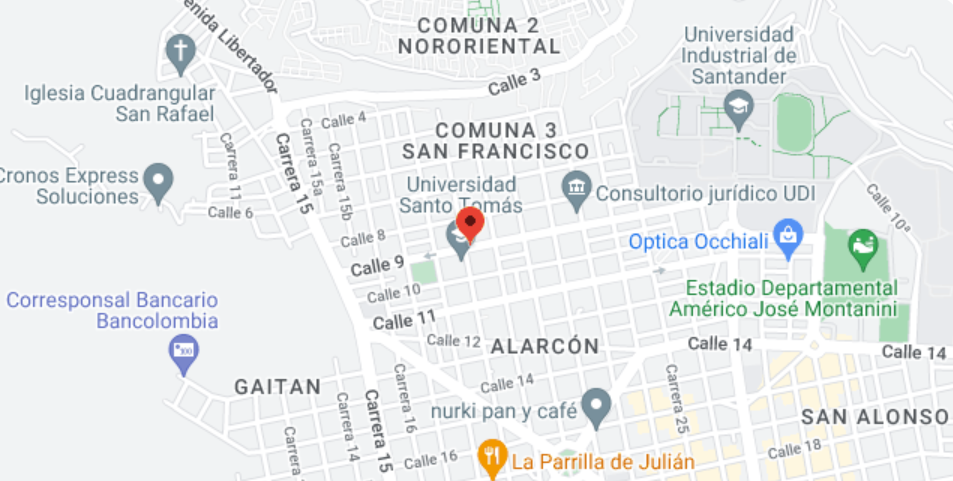
\includegraphics[width=0.8\textwidth]{Imagenes/ubicacion1}
	\caption{Fuente: Google Maps, Coordenadas: \textbf{Log:} -73.127821, \textbf{Lat:} 	
		7.137223.}
	\label{fig:mesh1}
\end{figure}

\subsection{Delimitación del sector}

\begin{itemize}
	\item Norte: Calle 9.
	\item Sur: Carrera 19.
	\item Oriente: Carrera 20.
	\item Occidente: Calle 10.
\end{itemize} 

\subsection{Amoblamiento urbano}

El sector cuenta con arbolización moderada, los elementos de señalización vial y ubicación geográfica son suficientes.

\subsection{Normatividad urbanística}

Conforme al Plan de Ordenamiento Territorial, aprobado mediante acuerdo N° 011 de 2014  `Por el cual se adopta el Plan de Ordenamiento Territorial de segunda generación del Municipio de Bucaramanga 2014 - 2027".

\subsubsection{Usos}

De acuerdo con la consulta del POT, el predio se encuentra ubicado en una zona comercial y de servicios livianos o al por menor, como se puede observar en la Figura No. \ref{fig:Usos}.\\

\textbf{CAPITULO 1°. ÁREAS DE ACTIVIDAD.}

\textbf{Articulo 325°. Definición de áreas de actividad.} Las áreas de actividad delimitan zonas en los suelos urbanos y de expansión urbana, en as cuales se orienta y/o fortalece la vocación del sector a partir de la asignación de los usos que se permiten, restringen y/o prohíben en dichos suelos, determinando las condiciones normativas para su desarrollo.

\textbf{Articulo 326°. Condiciones generales de la clasificación de áreas de actividad.} El presente Plan de Ordenamiento Territorial establece para cada área de actividad los usos permitidos, así como las condiciones para el desarrollo de cada uno de estas según la unidad de uso, su intensidad, tamaño, escala de cobertura y medidas para control de impactos urbanísticos, de conformidad con la clasificación consignada en los cuadros anexos N° 01 al 03.

\textbf{2. Zona comercial y de servicios livianos o al por menor (C-2).} Zonas destinadas al desarrollo de uso comercial especializado y venta de servicios generales y empresariales, en las diferentes escalas.

\begin{figure}[!h]
	\centering
	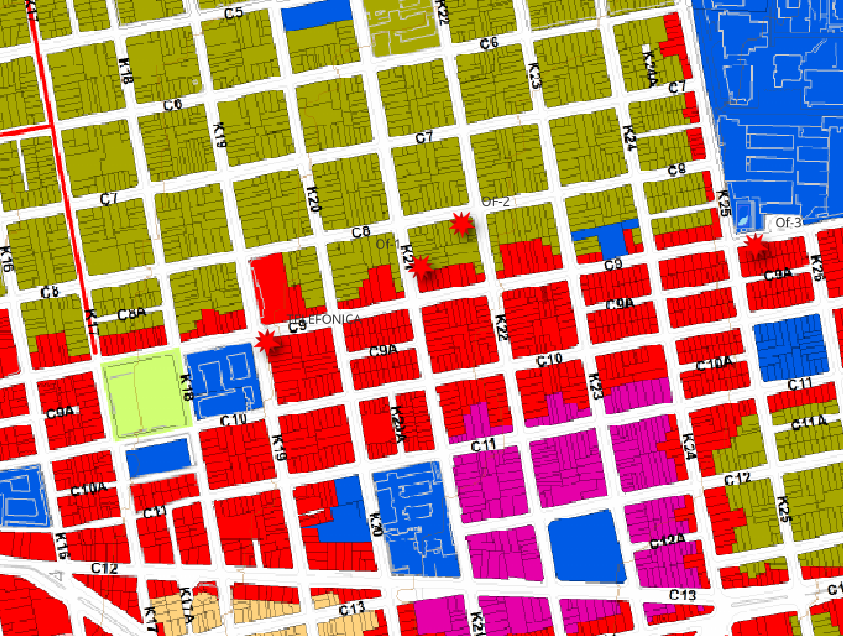
\includegraphics[width=0.8\textwidth]{Norma/AreaAc}
	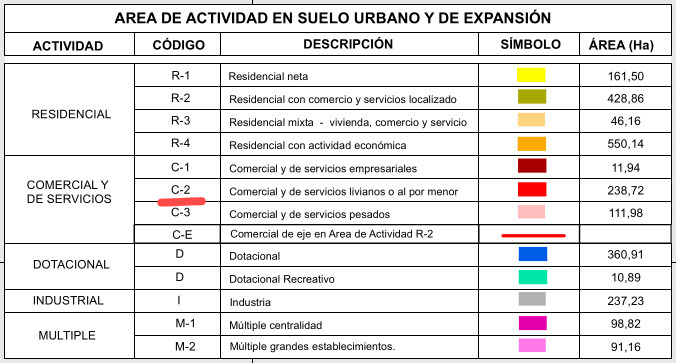
\includegraphics[width=0.8\textwidth]{Norma/AreaAcL}
	\caption{Fuente: Plano Áreas de actividad, Formulados POT}
	\label{fig:Usos}
\end{figure}

%\begin{center}
%
%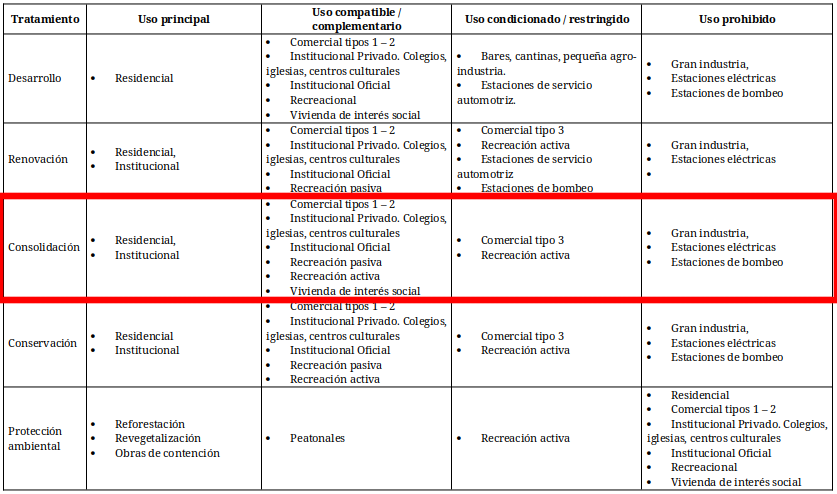
\includegraphics[width=\textwidth]{Norma/Usos1}\\
%\includegraphics[width=\textwidth]{Norma/Usos2}\\
%\includegraphics[width=\textwidth]{Norma/Usos3}\\
%\includegraphics[width=\textwidth]{Norma/Usos4}\\
%
%\end{center}

%\begin{description}
%	\item[Altura:] Resultante de aplicar la Norma.
%	\item[IO:] Resultante.
%	\item[IC:] 5.
%	\item[Antejardín:] 2 m.
%	\item[Aislamiento Posterior:] 2/5 de la altura promedio en metros de las edificaciones que se aíslan. La dimensión de
%	aislamiento no puede ser menor a 6.00 metros. En predios cuya geometría irregular no permita definir claramente la localización del aislamiento posterior, éste no se exige. En tales casos, se debe resolver el empate volumétrico con los aislamientos posteriores previstos en los predios vecinos, a través de patios. (Ver 2.2.2.1.3. Empates de aislamientos posteriores en el Tratamiento de Renovación Urbana) 
%%	\item[Patios:] $4 m^{2}$. 
%	\item[Voladizos:] 0.6 m.
%%	\item[Garajes:] 1 por cada 2 viviendas.
%	\item[Tratamiento:] Renovación Urbana.
%	\item[Área de actividad:] Área de actividad Estructuraste - AAE - Receptora de vivienda de interés social.
%	\item[Modalidad:] Urbanística.
%%	\item[Zona:] Residencial con zonas delimitadas de comercio y servicios.
%\end{description}


\subsubsection{Tratamiento}

%De acuerdo con la consulta del EOT, el predio se encuentra ubicado en una zona con tratamiento de Renovación urbana modalidad de redesarrollo, como se puede observar en la Figura No. \ref{fig:tratamiento}.\\

De acuerdo con la consulta del POT, el predio se encuentra ubicado en una zona de tratamiento de Reactivación. \\

\textbf{SUBTITULO 2°. TRATAMIENTOS URBANÍSTICOS:} \\

\textbf{Articulo 198°. Definición de tratamientos urbanísticos.} Los tratamientos urbanísticos orientan las
intervenciones que se pueden realizar en el territorio, atendiendo las características físicas de cada
zona y su función dentro del modelo territorial, a partir de la cual se establecen las normas urbanísticas
que definen un manejo diferenciado para los distintos sectores del suelo urbano y de expansión6n urbana.
Para el municipio de Bucaramanga se definen los siguientes tratamientos urbanísticos:
\begin{itemize}
	\item 1. Desarrollo.
	\item 2. Consolidación.
	\item 3. Renovación urbana
	\item 4. Mejoramiento integral.
	\item 5 Conservación.
\end{itemize}

\textbf{CAPITULO 3°. TRATAMIENTO DE RENOVACIÓN URBANA:} \\

\textbf{Articulo 216°.} Definición de tratamiento de renovación urbana y sus modalidades. Se aplica a
los sectores urbanizados y/o edificados de la ciudad que han sufrido procesos de deterioro de su
espacio público o de sus inmuebles y cambios en los usos originales; por ende, requieren acciones
integrales para la rehabilitación o transformación6n del espacio publico y/o de las construcciones para
aprovechar su potencial. Igualmente aplica en sectores que presentan aprovechamientos muy bajos
en relación con su potencial, por ende se permite que los predios tengan una mayor densificación,
garantizando coherencia entre la intensidad del uso del suelo y el sistema de espacio público. Este
tratamiento tiene dos (2) modalidades.\\

\textbf{2. Reactivación (TRA).} Se aplica a sectores en los cuales se promueve el cambio de las estructuras
en el interior de los predios con el fin de propiciar la densificación de las zonas en que se ubican y un
mejoramiento progresivo del espacio público, conservando la estructura o trazado de los bienes de
uso público, promoviendo la cualificación del sistema de espacio público en coherencia con la
intensidad del uso del suelo, y estimulando la generación de nuevos elementos arquitectónicos y
naturales de los bienes de propiedad privada.
La modalidad de Re activación (TRA) tiene tres (3) sub modalidades:
b. Reactivación 2 (TRA-2). Aplica en sectores donde se permite una mayor densificación de los predios, propiciando englobes y buscando mayor coherencia entre las intensidades de use del suelo y densidades edilicias con el sistema de espacio publico que las soporta.


%\textbf{Artículo 254 B. Tratamiento de Renovación Urbana} Son las determinaciones del componente urbano del Plan de Ordenamiento Territorial, que están encaminadas a recuperar y/o transformar las áreas ya desarrolladas de las ciudades, entre otros fines, para, detener los procesos de deterioro físico y ambiental de los centros urbanos; promover el aprovechamiento intensivo de la infraestructura publica existente; impulsar la densifican racional de áreas para vivienda y otros usos, o garantizar la conveniente rehabilitación de los bienes históricos y culturales, todo con miras a una utilización mas eficiente de los inmuebles urbanos y con mayor beneficio para la comunidad. Este tratamiento podrá desarrollarse mediante las modalidades de reactivación y redesarrollo.\\

\begin{figure}[!h]
	\centering
	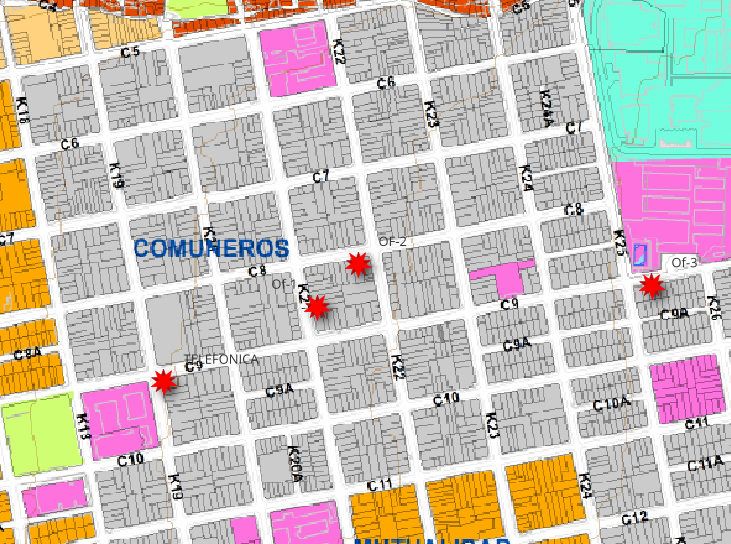
\includegraphics[width=\textwidth]{Norma/Tratamiento}
	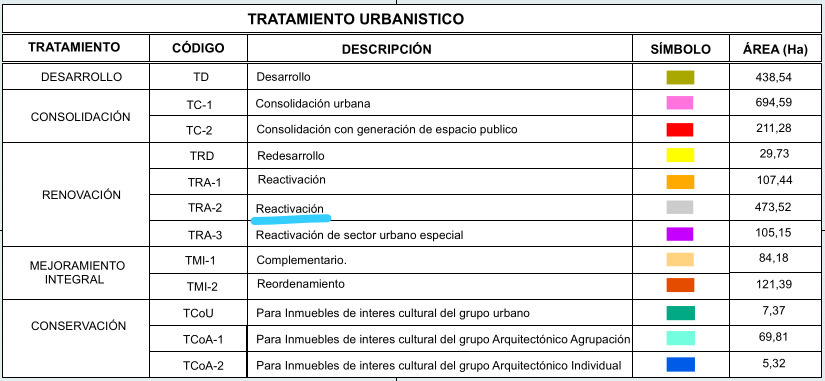
\includegraphics[width=\textwidth]{Norma/TratamientoL}
%		\includegraphics[width=0.45\textwidth]{Norma/TratamientoG}
	\caption{Fuente: Tratamiento Urbanístico POT}
	\label{fig:tratamiento}
\end{figure}

\begin{figure}[!h]
	\centering
	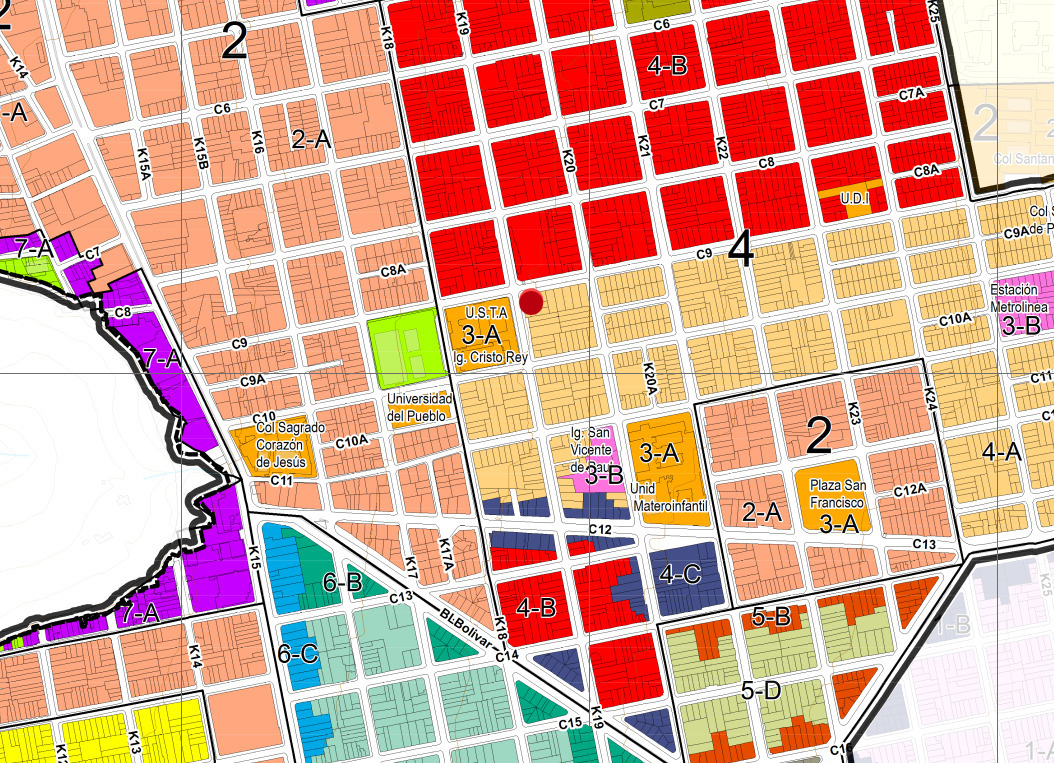
\includegraphics[width=0.7\textwidth]{Norma/Edificabilidad}
	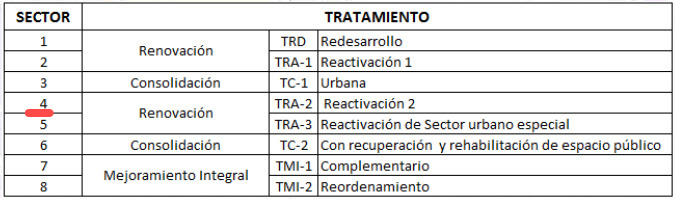
\includegraphics[width=0.7\textwidth]{Norma/Edificabilidad1}\\	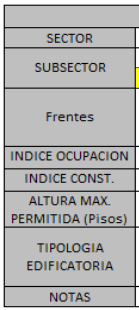
\includegraphics[width=0.1\textwidth]{Norma/Edificabilidad3}
	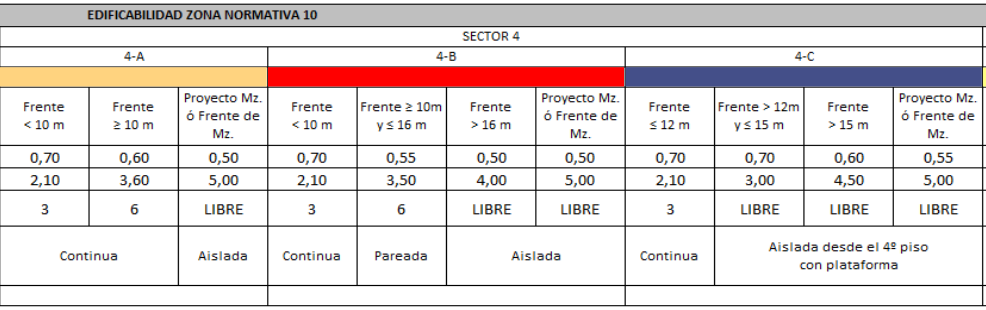
\includegraphics[width=0.7\textwidth]{Norma/Edificabilidad2}\\
	\caption{Fuente: Edificabilidad POT}
	\label{fig:tratamiento}
\end{figure}




\begin{figure}[!h]
	\centering
	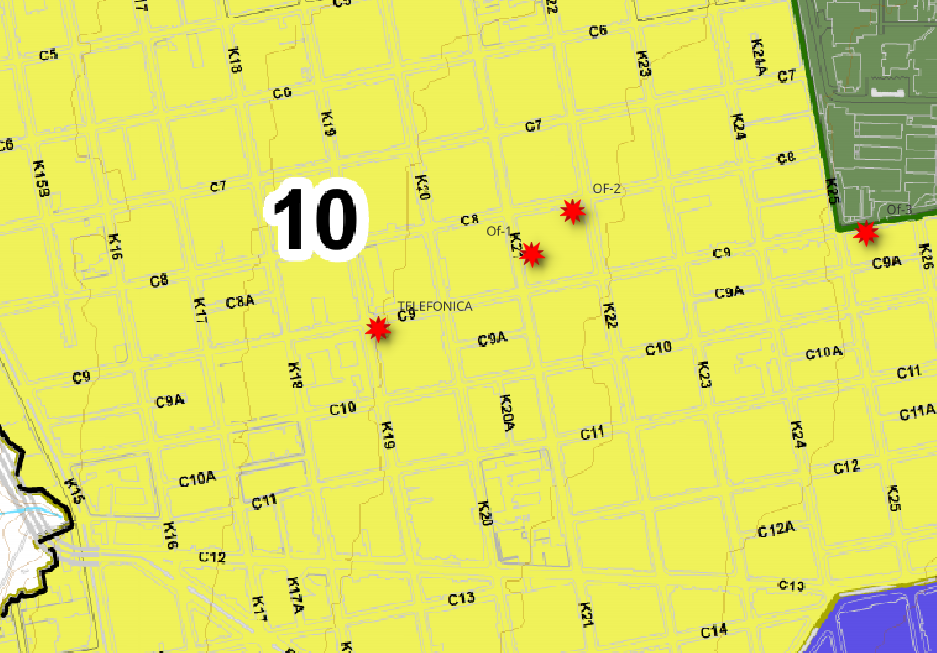
\includegraphics[width=0.5\textwidth]{Norma/sectornormativo}
	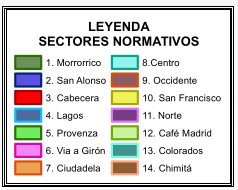
\includegraphics[width=0.3\textwidth]{Norma/sectornormativo1}
	%		\includegraphics[width=0.45\textwidth]{Norma/TratamientoG}
	\caption{Fuente: Sector Normativo POT}
	\label{fig:tratamiento}
\end{figure}

\begin{center}
	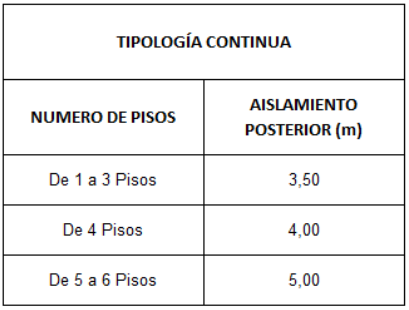
\includegraphics[width=0.3\textwidth]{Norma/Edificabilidad4}
\end{center}

%\subsubsection{Norma urbanística}

%El inmueble presenta la siguiente norma urbanística:

\begin{center}
%\includegraphics[width=\textwidth]{Norma/Tratamiento1}\\
%\includegraphics[width=\textwidth]{Norma/Tratamiento2}\\
%\includegraphics[width=\textwidth]{Norma/Tratamiento3}\\
%\includegraphics[width=\textwidth]{Norma/Tratamiento4}\\
%\includegraphics[width=\textwidth]{Norma/Tratamiento5}\\
%\includegraphics[width=\textwidth]{Norma/Tratamiento6}\\
\end{center}



\subsection{Servicios Públicos}

El sector cuenta con servicios públicos de energía, acueducto, gas natural, telefonía fija, recolección de basuras y alcantarillado.

\subsection{Vías publicas de acceso}

\subsubsection{Principales}

Las vías principal más importantes de la zona corresponden a la carrera 15 y calle 3.  Se desplaza un alto flujo vehicular y se desarrolla la mayor actividad comercial de la zona, en general se encuentra en buen estado de conservación.	

\subsubsection{Secundarias}

 Cuenta con vías para acceder al sector, como  la  Calle 9 y Carrera 19. Se encuentran en buen estado de conservación.

\subsubsection{Transporte publico}

El servicio de transporte público es suministrado principalmente por  buses, busetas, colectivos y taxis, que comunican a los diferentes puntos del municipio.

\subsection{Topografía}

El inmueble se encuentra en un sector con topografía Plana.%(Ligeramente inclinada, inclinada y escarpada).

\subsection{Estrato socioeconomico}

 Se aclara que el estrato aplica exclusivamente si el inmueble es de uso residencial, de acuerdo con lo establecido en la Ley 142 de 1994.

%\subsection{Legalidad de la Urbanización}
%
%La Urbanización se encuentra legalizada según el Decreto 443 de 2011

\section{Características Físicas}

\subsection{Tipo de bien inmueble}

Lote de terreno junto con la construcción sobre el levantada.

\subsection{Características del terreno}


\begin{tabular}{ l l }
   
%\textbf{LOCAL NUMERO CIENTO CUARENTA (140)}
   
    Forma: & Regular\\
   Área medida en sitio: & 224,58 $m^{2}$\\
  % Área catastro: & 611 $m^{2}$\\
   Área en documentos: & 260 $m^{2}$\\
   Frente: & 13 m\\
  Fondo: & 20 m\\
   Relación Frente - Fondo: & 1.54\\
   Topografía: & Plana\\
   %Forma: & Regular\\
   
\end{tabular}

\paragraph{Nota 1:} Se encuentra una diferencia, entre el área en documentos y el área medida en sitio, se adopta el área en documentos jurídicos.

%\paragraph{Nota 2:} No se pudo medir el perímetro del terreno dado que no se tuvo acceso directo al bien inmueble, sin embargo se logro identificar de forma correcta el mismo.

\subsubsection{Linderos}

	
%\textbf{\textbf{LOCAL NUMERO CIENTO CUARENTA (140):}}
\begin{itemize}
	
	\item \textbf{NORTE:} En 20 metros con la calle 9A.\\
	\item \textbf{SUR:} En 20 metros con propiedad de Rufino Serrano. \\
	\item \textbf{ORIENTE:} En 13 metros, con propiedad de Severo Suarez.\\
	\item \textbf{OCCIDENTE:}  En 13 metros, con la carrera 19.\\
\end{itemize}




\paragraph{Fuente}: \EscrituraAportada.

%\paragraph{Nota: } En atención a la solicitud del cliente, se procederá a adoptar el área calculada a partir de los linderos descritos en la escritura. Se ha identificado que en los documentos  no se encuentra el área totalizada. Por lo tanto, se recomienda llevar a cabo una actualización de cabida y linderos.   

\subsection{Afectaciones}

\subsubsection{Ambientales}

No se encuentran problemas que impacten de forma negativa el bien inmueble, como aguas negras, rellenos sanitarios y problemas de basuras.

\subsubsection{Servidumbres, cesiones y afectaciones viales}

El predio no cuenta con servidumbres, cesiones y afectaciones viales que restrinjan su uso.

\subsection{Servicios públicos}
	
%\paragraph{En el predio}

	El Predio cuenta con servicios públicos instalados de energía y acueducto.
\subsection{Características de la Construcción}

%Aunque el bien inmueble cuenta con una construcción, no se obtuvo acceso a esta.
\subsubsection{Datos generales}
%
\begin{tabular}{ l l }
%	
	Pisos: & 3.\\
	Sótanos: & 1.\\
	Vetustez: & 27 años \\
	Vida útil: & 100 años \\
	Vida restante: & 73 años \\
%	
\end{tabular}
%
\subsubsection{Croquis de la construcción}
%
\textbf{Áreas encontradas en la visita técnica.} \\
%
%
\begin{center}
	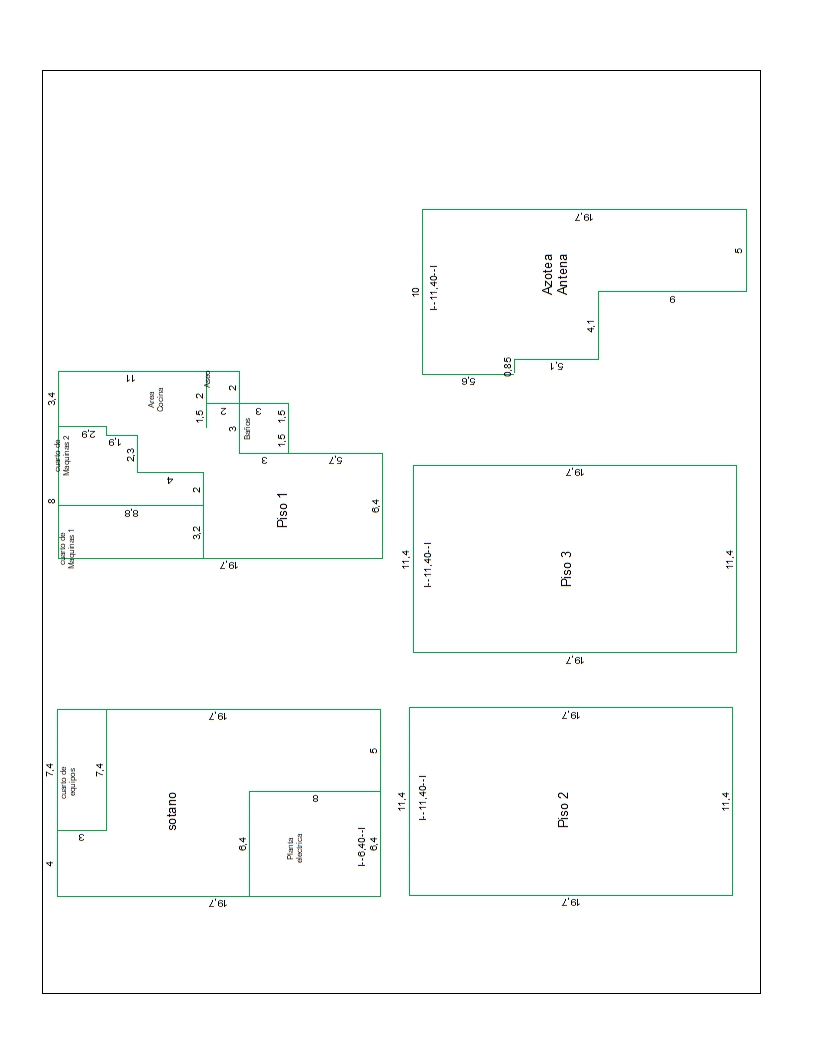
\includegraphics[width=0.8\textwidth]{Imagenes/PLANO}
\end{center}
%
\paragraph{Nota 1:} Las mediciones realizadas en sitio se consideran aproximadas de acuerdo con la exactitud del dispositivo utilizado, estas medidas no corresponde a un levantamiento arquitectónico.
%
\subsubsection{Área construida}
%
\begin{center}
%	
	\begin{tabular}{ ||l| |l| |l|| }
%		
	\textbf{Identificación} & \textbf{Área} & \textbf{Destinación} \\
%		Sotano & $100 m^{2}$ & Comercial \\
		Terreno & $260 m^{2}$ & Oficinas y Área técnica. \\
		Sotano & $259,54 m^{2}$ & Planta eléctrica.  \\
		Piso 1 & $244,38 m^{2}$ & Planta eléctrica.  \\
		Piso 2 & $239,66 m^{2}$ & Oficinas.  \\
		Piso 3 & $239,66 m^{2}$ & Oficinas.  \\
%		Bodega & $17.42 m^{2}$ & Oficinas  \\
%		Ramada & $46.41 m^{2}$ & Oficinas  \\
%		Planta eléctrica & $33.64 m^{2}$ & Oficinas  \\
	\end{tabular}
\end{center}
%
\paragraph{Nota} 
No se tuvo acceso al segundo y tercer piso del edificio; por lo tanto, las medidas se han tomado a partir de los planos aportados. 
%%El predio presenta un ampliación de $30 m^{2}$, sobre el aislamiento posterior, la cual no se tubo en cuenta dentro de la valoración, ya que esta no es susceptible de legalizar.
%
\subsubsection{Dependencias}
%
\begin{description}
%
\item[Sotano:] Planta eléctrica.	
\item[Piso 1:] Recepción, Oficinas, cuarto útil, baño, cocina, Área Técnica. 
\item[Piso 2:] Área de oficinas, área técnica, hall y baños.
\item[Piso 3:] Área de oficinas y baños.
%%\item[Piso 4:] Espacio disponible para oficinas.
%%\item[Piso 5:] Terraza, tanque de agua.
%
\end{description}
%
\subsubsection{Estado de conservación}
%
\paragraph{Estructura}
%
 Se encuentra  en buen estado de conservación. No se observan fisuras, humedad o movimiento de esta por asentamiento o movimientos del terreno.	
%
\paragraph{Acabados}
%
Se encuentra  en buen estado de conservación con bajo mantenimiento, no se observan remodelaciones ni mantenimientos en pisos, paredes, y techos.
%
\subsubsection{Especificaciones constructivas}
%
\begin{tabular}{ l l }
%
   Cimentación: & Se presumen zapatas aisladas en concreto reforzado.\\
   Estructura: & Tradicional.\\
%/Muros de carga./ Industrializada.\\
  Muros: & Pañete estuco y pintura.\\
  %Entre placas: & Concreto reforzado.\\
  Cubierta: & Placa de concreto impermeabilizada.\\ %plástica /metálica /barro.\\
   Fachada: & Graniplast.\\
   Cielo raso: & Icopor con estructura metálica.\\
%          
 \end{tabular}
%
%\subsubsection{Acabados generales}
%
%\begin{tabular}{ l l }
%
%   Cielo razo: & Placa de concreto, paneles de fibrocemento.\\
%   %Drywall, Estuco y pintura, Carraplast  \\
%   Pisos: & Baldosa cerámica, Cemento afinado.\\ %Baldosa cerámica, Porcelanato, madera natural, Cemento afinado, Tablón de gres, y Machimbre\\
%   Muros: & Estuco y pintura.\\ %Ladrillo a la vista, Pañete y pintura.\\
%   Guarda escobas: & Baldosa Cerámica.\\ %Baldosa, Madera laminada, Madera natural, \\
%   Puertas exteriores: & Metálicas.\\
%   %Madera aglomerada, Aluminio, Vidrio templado, Metal\\
%   Puertas Interiores: & Madera.\\ 
%   %aglomerada Aluminio, Vidrio templado, Madera\\
%          
% \end{tabular}
 
% \subsubsection{Acabados en Bodega} 

% \begin{tabular}{ l l }

%    Pisos: & Cemento afinado\\
%    Cielo razo: & Paneles en aluminio e icopor.\\
%   %Madera laminada, Baldosa , Porcelanato, madera natural, Cemento afinado\\
%    Muros: & Pañete y pintura.\\
%    Puertas exteriores: & Metálicas 
%   %Ladrillo a la vista, Pañete y pintura.\\
%   %Muebles: & Lamina de madera aglomerada, acrílico, acero inoxidable.\\
%   Mesón: & Concreto enchapado.\\
%   %Granito, acero inoxidable, Concreto enchapado.\\
%   Lava platos: & Sin lavaplatos.\\
%   %Electrodomésticos fijos: & Extractor de olores, Horno, Estufa.\\
%             
% \end{tabular}
% 
%\subsubsection{Acabados en baños} Se encuentra en mal estado de conservación lo que se observa:
%
%\begin{tabular}{ l l }
%
%   Pisos: & Baldosa cerámica.\\
%   Muros: & Cerámica, Pañete y pintura.\\
%   %Muebles: & Lamina de madera aglomerada, acrílico, acero inoxidable.\\
%   Sanitario: & Cerámica.\\
%   Lavamanos: & Sin Lavamanos.\\
%   %vidrio templado, Baldosa cerámica. \\ 
%   %Accesorios: & Cerámica.\\
%   %Plástico, acero inoxidable, cerámica.\\
%   %Divisiones: & Vidrio templado, Acrílico\\   %Divisiones: & Vidrio templado, Acrílico\\
%   %Especiales: & Tina, Jacuzzi, Sauna, Cabina de hidromasaje.\\
%  
%  \end{tabular}
% 

%\subsubsection{Condiciones de iluminación y ventilación}
%
%El predio cuenta con una buena iluminación y buena ventilación.
	
\section{Alcance del avalúo}

El avalúo tiene por objeto hallar el valor de mercado para el bien inmueble definido e identificado en el presente informe y la renta total del bien inmueble respecto a la solicitud presentada.

\section{Condiciones restrictivas y afectaciones}

\subsection{Problemas de estabilidad y suelos}

No se encuentran problemas de inestabilidad del suelo.

\subsection{Impacto ambiental y condiciones de salubridad}

El predio no se encuentra en una zona que se vea afectada por condiciones ambientales o de salubridad.

%\begin{figure}[!h]
%	\centering
%	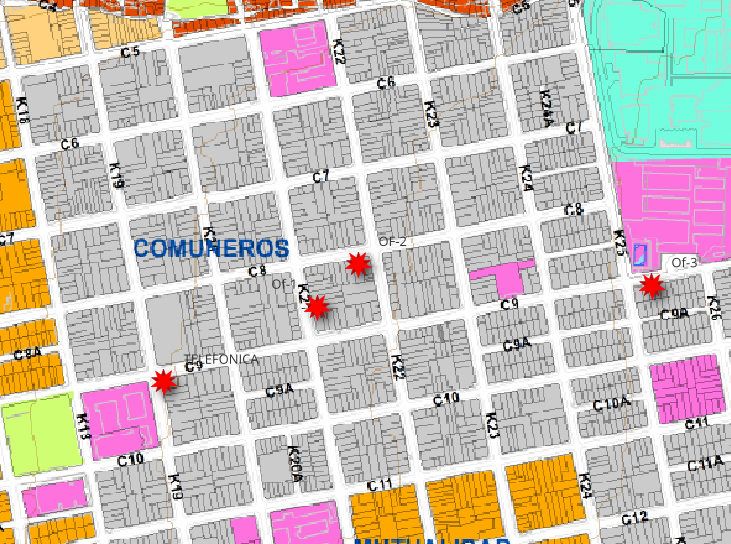
\includegraphics[width=0.8\textwidth]{Norma/Tratamiento}
%			\includegraphics[width=0.45\textwidth]{Norma/TratamientoG}
%	\caption{Fuente: Tratamiento Urbanístico PBOT}
%	\label{fig:Proteccion}
%\end{figure}

%\includegraphics[width=\textwidth]{Norma/Ambiental1}\\
%\includegraphics[width=\textwidth]{Norma/Ambiental2}\\
%\includegraphics[width=\textwidth]{Norma/Ambiental3}\\

\subsection{Seguridad}

La zona no presenta problemas de inseguridad.

\section{Condiciones generales}

Para el presente informe se tuvieron en cuenta los siguientes supuestos:

\begin{itemize}
	
%	\item El inmueble presenta un cuarto técnico, que puede representar dificultad para la comercialización ya que se debe desmontar sin afectar la conectividad existente.
%	\item Dentro del análisis que se adelanta se adopta el área calculada a partir de los linderos descritos en la escritura y no se tendrá en cuenta dentro de la valoración la Ramada por petición del solicitante.
%	\item Se recomienda llevar a cabo una actualización de cabida y linderos.
    %\item De igual manera que en el análisis anterior, para el estudio de renta parcial se asume el limite inferior, ya que los equipos instalados en la vivienda, generan incomodidades en términos de mantenimientos, ruido y de mas factores que disminuyen el publico objetivo.
    %\item Se asigna un valor diferencial para la bodega, teniendo en cuenta que los acabados presentes son diferentes al resto de la vivienda.
    \item No se aporto certificado de tradición y libertad actualizado.
	\item Los análisis y resultados solamente se ven restringidos por las hipótesis y condiciones restrictivas que se describen en el informe.
	\item La medida de las áreas construidas se realiza a partir de los planos aportados por el cliente, las cuales fueron validadas en sitio.
	
\end{itemize}

\section{Declaración de cumplimiento}

\begin{itemize}
	\item La presente valuación se realizó siguiendo las disposiciones en cuanto a metodología establecidas por el Instituto Geográfico Agustín Codazzi –IGAC– mediante Resolución número Seiscientos Veinte (620) del 23 de septiembre de 2008, con el objeto de establecer el valor comercial en el mercado actual, del inmueble que en este informe se ha descrito.
	\item El contenido del presente informe de avalúo ha tenido en cuenta parámetros establecidos en las NTS S 03 “Contenido de Informes de Valuación” y la NTS I 01 “Contenido de Informes de Valuación de Bienes Inmuebles Urbanos”.
	\item El presente informe ha sido elaborado de conformidad con las normas del “Código Colombiano de Ética del Avaluador”, del Registro Nacional de Avaluadores de la ANA y de acuerdo a los parámetros exigidos por la entidad Gubernamental Autorregulación Nacional de Avaluadores.
	\item Las descripciones de hechos presentadas en el informe son correctas hasta donde el Valuador alcanza a conocer.
	\item Los análisis y resultados solamente se ven restringidos por las hipótesis y condiciones restrictivas que se describen en el informe.
	\item El valuador, directivos y asociados de GEOVALORES, no tienen intereses financieros ni de otra índole en el inmueble avaluado, ni vínculos de naturaleza alguna con sus propietarios, más allá de los derivados de la contratación de nuestros servicios profesionales.
	\item La valuación se llevó a cabo conforme a un código de ética y normas de conducta.
	\item El Valuador ha cumplido los requisitos de formación de su profesión.
	\item El Valuador tiene experiencia en el mercado local y la tipología de bienes que se están valorando.
	\item El Valuador ha realizado una visita personal al inmueble y nadie, con excepción de las personas especificadas en el informe, ha proporcionado asistencia profesional en la preparación del informe.
	
\end{itemize}

\section{Responsabilidad del Valuador}

\begin{itemize}
	\item El valuador no sera responsable por aspectos de naturaleza legal que afecten el bien inmueble, a la propiedad valuada o el titulo legal de la misma (Escritura).
	\item El valuador no revelara información sobre la valuación a nadie distinto de la persona natural o jurídica que solicito el encargo valuatorio y solo lo hará con autorización escrita de esta, salvo en el caso en que el informe sea solicitado por una autoridad competente.
	\item El informe de valuación es confidencial para las partes, hacia quien esta dirigido o sus asesores profesionales, para el propósito especifico del encargo; no se acepta ninguna responsabilidad ante ninguna tercera parte, el valuador no acepta ninguna responsabilidad por la utilización inadecuada del informe.
	\item El presente informe parte de la buena fe del solicitante en relación con la veracidad en el suministro de la información, con lo cual queda salvada la responsabilidad del valuador, hasta donde fue posible su verificación.
	\item El presente estudio no comprende en modo alguno la valuación de otros bienes tangibles o intangibles que pudieran estar vinculados de alguna forma a las instalaciones físicas de los inmuebles, como por ejemplo “GoodWill”, primas, la valuación de la empresa en marcha o la rentabilidad de la participación tenida sobre la operación del negocio.
	
\end{itemize}

\section{Declaración no existencia de conflicto de interés}

Dando cumplimiento a la política de Conflicto de Intereses de COLOMBIA\\ 
TELECOMUNICACIONES S.A. ESP BIC., yo Omar Salcedo Uriza identificado con C.C. No.80154037 a título personal y actuando en nombre y representación de la sociedad GEOVALORES NIT 900.738.463-1 declaro:

1. NO tener parientes en primer grado de consanguinidad (padres, hijos) y/o segundo grado de consanguinidad (hermanos) trabajando en alguna de las empresas del Grupo Telefónica, en empresas contratistas (proveedores, comercializadores etc.) del Grupo Telefónica o en empresas del sector de las telecomunicaciones.

2. NO tener parientes en tercer grado de consanguinidad (sobrinos) y/o cuarto grado de consanguinidad (primos) trabajando en alguna de las empresas del Grupo Telefónica, en empresas contratistas (proveedores, comercializadores etc.) del Grupo Telefónica y en especial con colaboradores que hacen parte del Proyecto de Venta de Inmuebles o en empresas del sector de las telecomunicaciones.

3. NO tener parientes en primer y/o segundo grado de afinidad (suegros y cuñados) trabajando en alguna de las empresas del Grupo Telefónica, en empresas contratistas (proveedores, comercializadores etc.) del Grupo Telefónica y en especial con colaboradores que hacen parte del Proyecto de Venta de Inmuebles o en empresas del sector de las telecomunicaciones.

4. NO tener parientes civiles (hijo adoptivo, padre adoptante) y/o mi esposo(a), o compañero(a) permanente trabajando en alguna de las empresas del Grupo Telefónica, en empresas contratistas (proveedores, comercializadores etc.) del Grupo Telefónica o en empresas del sector de las telecomunicaciones y en especial con colaboradores que hacen parte del Proyecto de Venta de Inmuebles.

5. NO tener actividades que pueden estar en competencia o conflicto con los productos y servicios ofrecidos por Telefónica, que son perjudiciales para a los mejores intereses de la compañía.

6. No existen a la fecha situaciones potenciales que puedan considerarse como posibles Conflictos de Interés
	

\section{Aspecto económico}

\subsection{Metodologías valuatorias empleadas}

\subsubsection{Método  de  comparación  o  de  mercado:}  	

Es  la  técnica  valuatoria  que busca  establecer  el  valor  comercial  del  bien,  a  partir  del  estudio  de  las  ofertas  o transacciones recientes, de bienes semejantes y comparables al del objeto de avalúo. Tales ofertas o transacciones deberán ser clasificadas, analizadas e interpretadas para llegar ala estimación del valor comercial.

\subsubsection{Método de capitalización de rentas o ingresos:}  

Es la técnica valuatoria que  busca  establecer  el  valor  comercial  de  un  bien,  a  partir  de  las  rentas  o  ingresos que  se  puedan  obtener  del  mismo  bien,  o  inmuebles  semejantes  y  comparables  por sus  características  físicas,  de  uso  y  ubicación,  trayendo  a  valor  presente  la  suma  de los  probables  ingresos  o  rentas  generadas  en  la  vida  remanente  del  bien  objeto  de avalúo, con una tasa de capitalización o interés.  


%\subsubsection{Método  de  costo  de  reposición:} 
%
%Es  el  que  busca  establecer  el  valor comercial del bien objeto de avalúo a partir de estimar el costo total de la construcción a precios de hoy, un bien semejante al del objeto de avalúo, y restarle la depreciación acumulada.  Al  valor  así  obtenido  se  le  debe  adicionar  el  valor correspondiente  al terreno.
%
%\subsubsection{Método   (técnica)   residual.:}  
%
%Es el   que   busca   establecer      el   valor comercial del bien, normalmente para el terreno, a partir de estimar el monto total de las ventas de un proyecto de construcción, acorde con la reglamentación  urbanística vigente  y  de  conformidad  con  el  mercado  del  bien  final  vendible,  en  el  terreno  objeto de avalúo. 
%
%Para encontrar el valor total del terreno se debe descontar al monto total de las ventas proyectadas,  los  costos  totales  y  la  utilidad  esperada  del  proyecto  constructivo.  Es indispensable que además de la factibilidad técnica y jurídica se evalúe la  factibilidad comercial del proyecto, es decir la real posibilidad de vender lo proyectado.

%\paragraph{Parágrafo}
%Este  método  (técnica)  debe  desarrollarse  bajo  el  principio  de  mayor  y mejor  uso,  según  el  cual  el  valor  de  un  inmueble  susceptible  de  ser  dedicado  a diferentes usos será el que resulte de destinarlo, dentro de las posibilidades legales y físicas,  al  económicamente  más  rentable,  o  si  es  susceptible  de  ser  construido  con distintas  intensidades  edificatorias,  será  el  que  resulte  de  construirlo,  dentro  de  las posibilidades  legales  y  físicas,  con  la    combinación  de  intensidades  que  permita obtener la mayor rentabilidad, según las condiciones de mercado.

\subsection{Justificación de las metodologías}

Se considera que la metodología utilizada es la más apropiada, por cuanto se encontraron ofertas de inmuebles similares o comparables que pudieron servir de punto de referencia, con las cuales se pudo determinar el Valor de Mercado del bien en estudio. 

\subsubsection{Memorias de cálculos}

Ver Anexos.

\subsubsection{Perspectivas de valorización}

Se consideran normales, de acuerdo con su ubicación relativa y tipología.

%\subsubsection{Concepto de garantía}

\newpage

\section{Valuación}

\begin{center}
	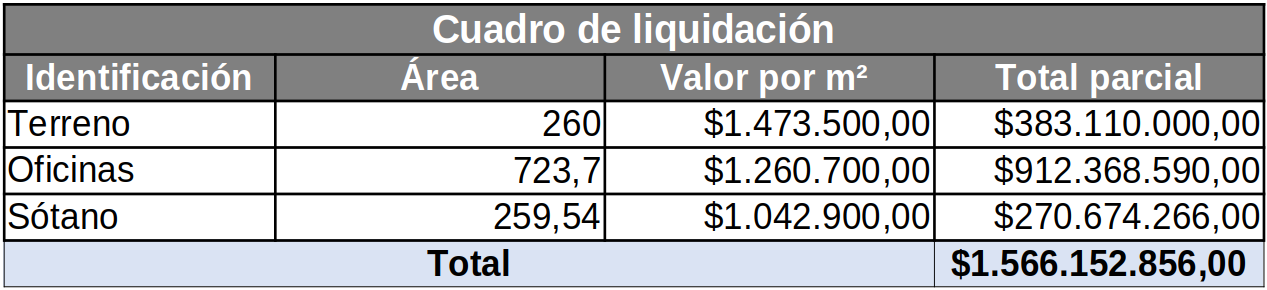
\includegraphics[width=\textwidth]{Imagenes/Valoracion1}
\end{center}

\paragraph{Son: } MIL QUINIENTOS SESENTA Y SEIS MILLONES CIENTO CINCUENTA Y DOS MIL OCHOCIENTOS CINCUENTA Y SEIS  PESOS MONEDA CORRIENTE.

\subsection{Nombre, cualificación profesional y firma del valuador}


	
\includegraphics[scale=0.2]{Imagenes/Firma}


Ing. Juan Palma\\
Perito - RAA: AVAL-1013620663

\section{Calculo de Valor de Renta Parcial Mensual}

\begin{center}
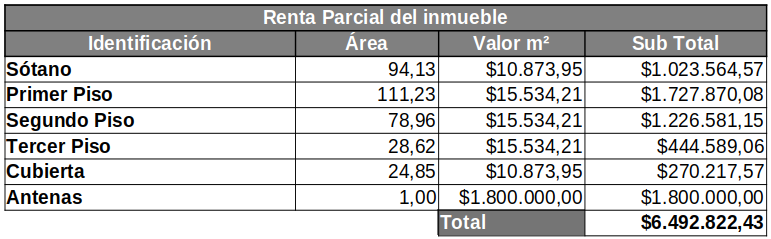
\includegraphics[width=\textwidth] {Imagenes/RentaParcial1}
\end{center}

\section{Calculo de Valor de Renta Total}

\begin{center}
	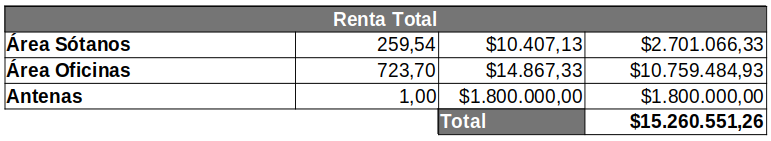
\includegraphics[width=\textwidth]{Imagenes/RentaTotal1}
\end{center}

\newpage

\section{Registro Fotográfico}

\begin{tabular}{ c c }
	
	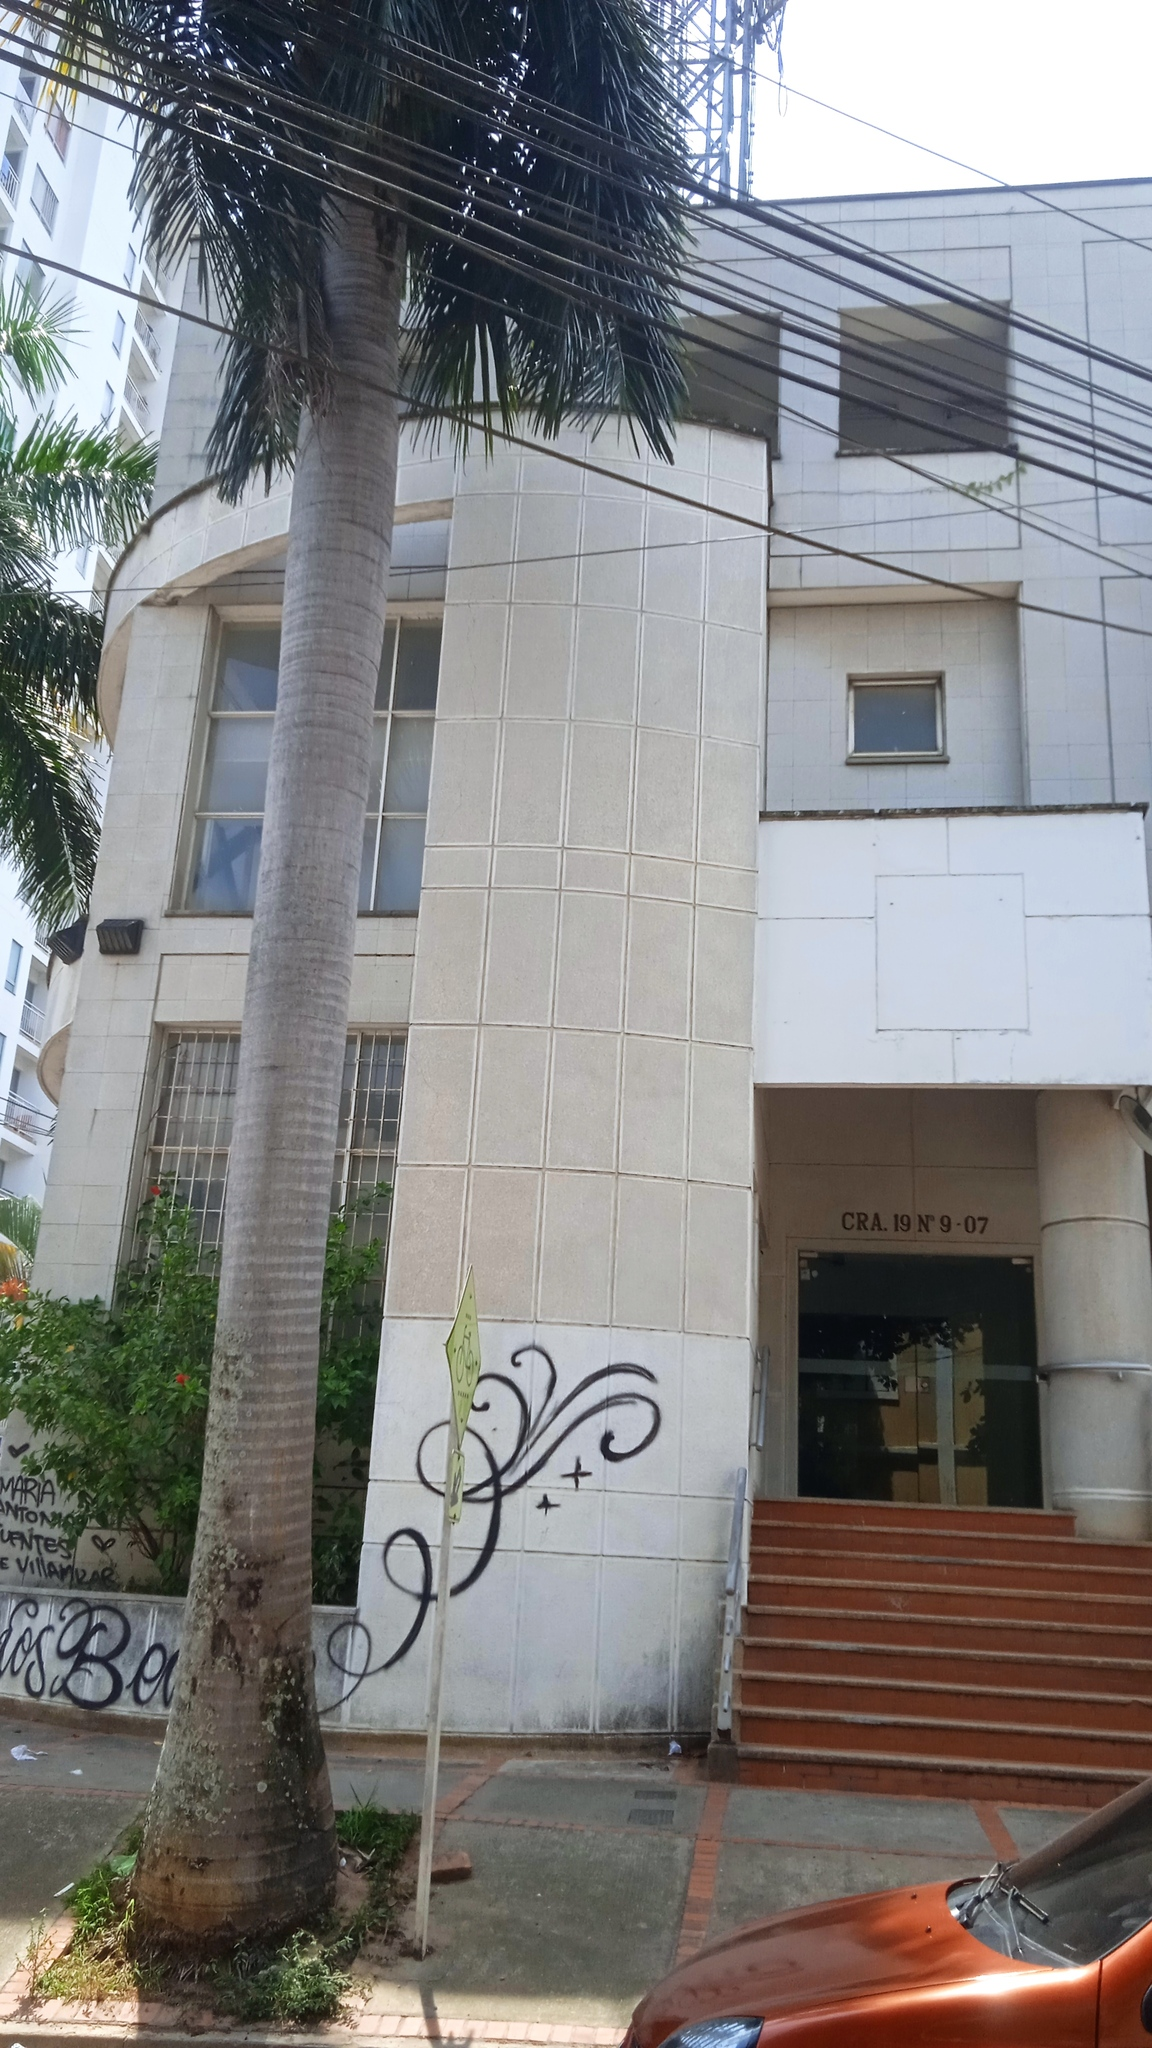
\includegraphics[width = 3 cm]{Imagenes/1} & 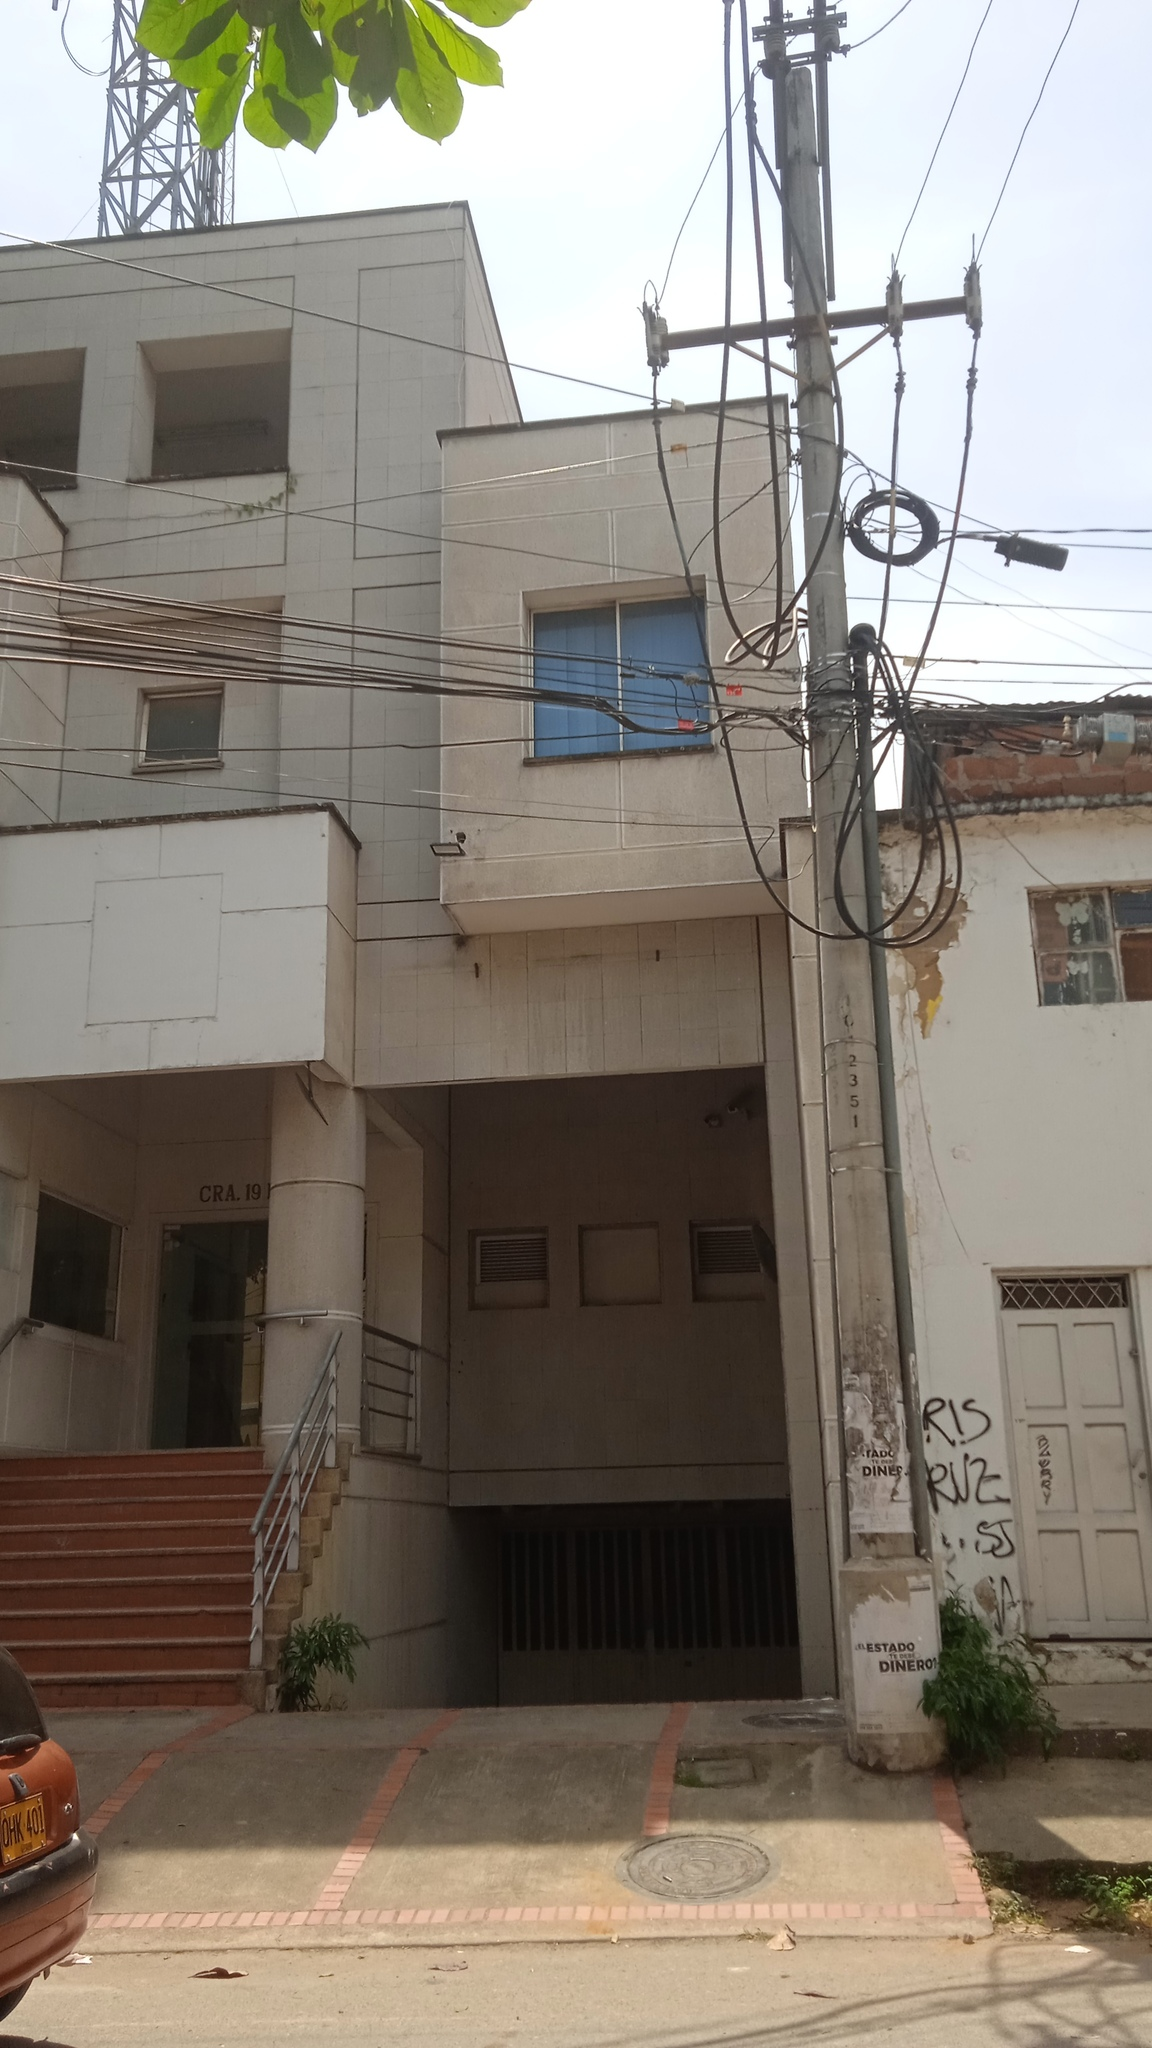
\includegraphics[width = 3 cm]{Imagenes/2} \\
	FACHADA  & FACHADA  \\
	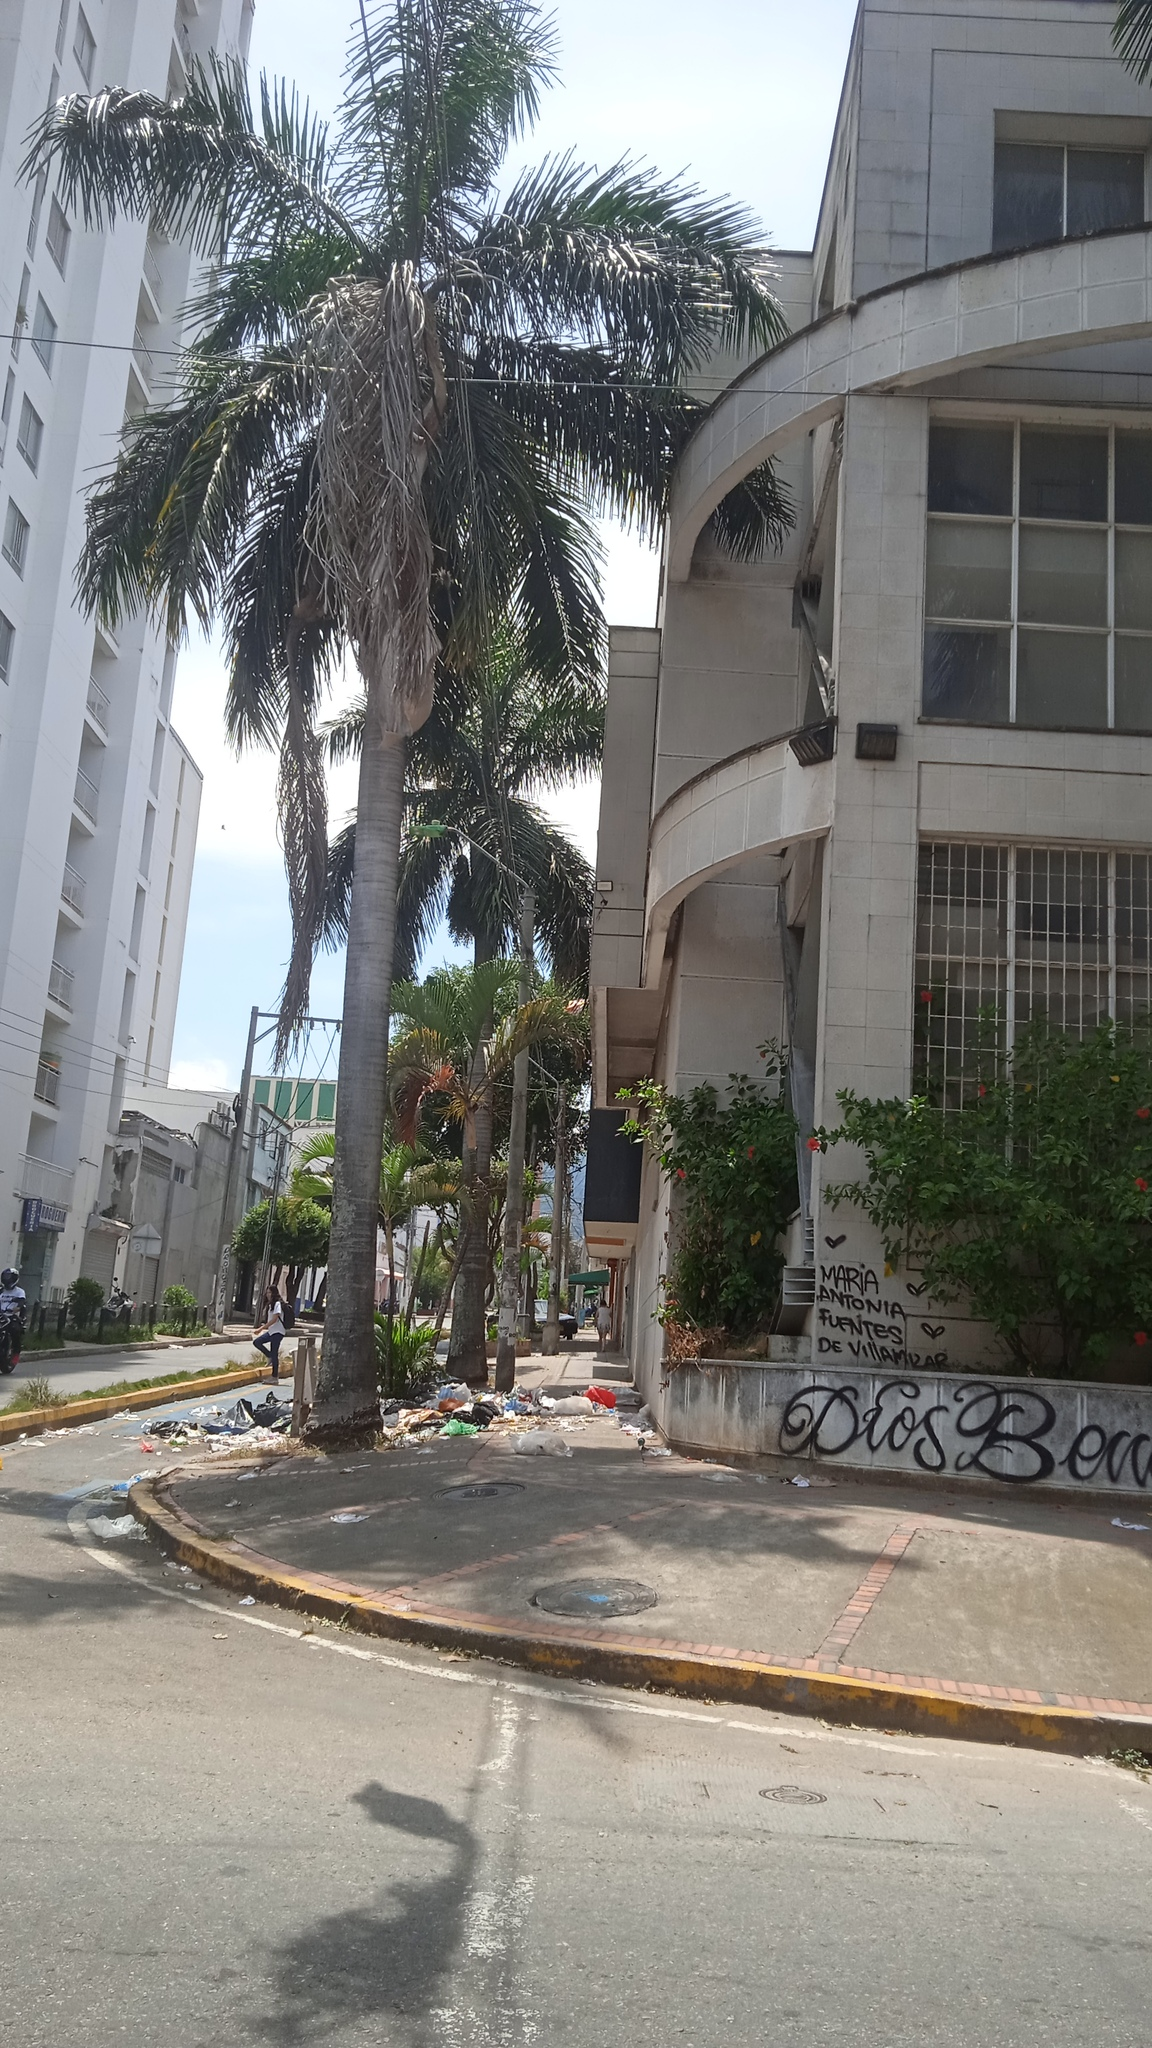
\includegraphics[width = 3 cm]{Imagenes/3} & 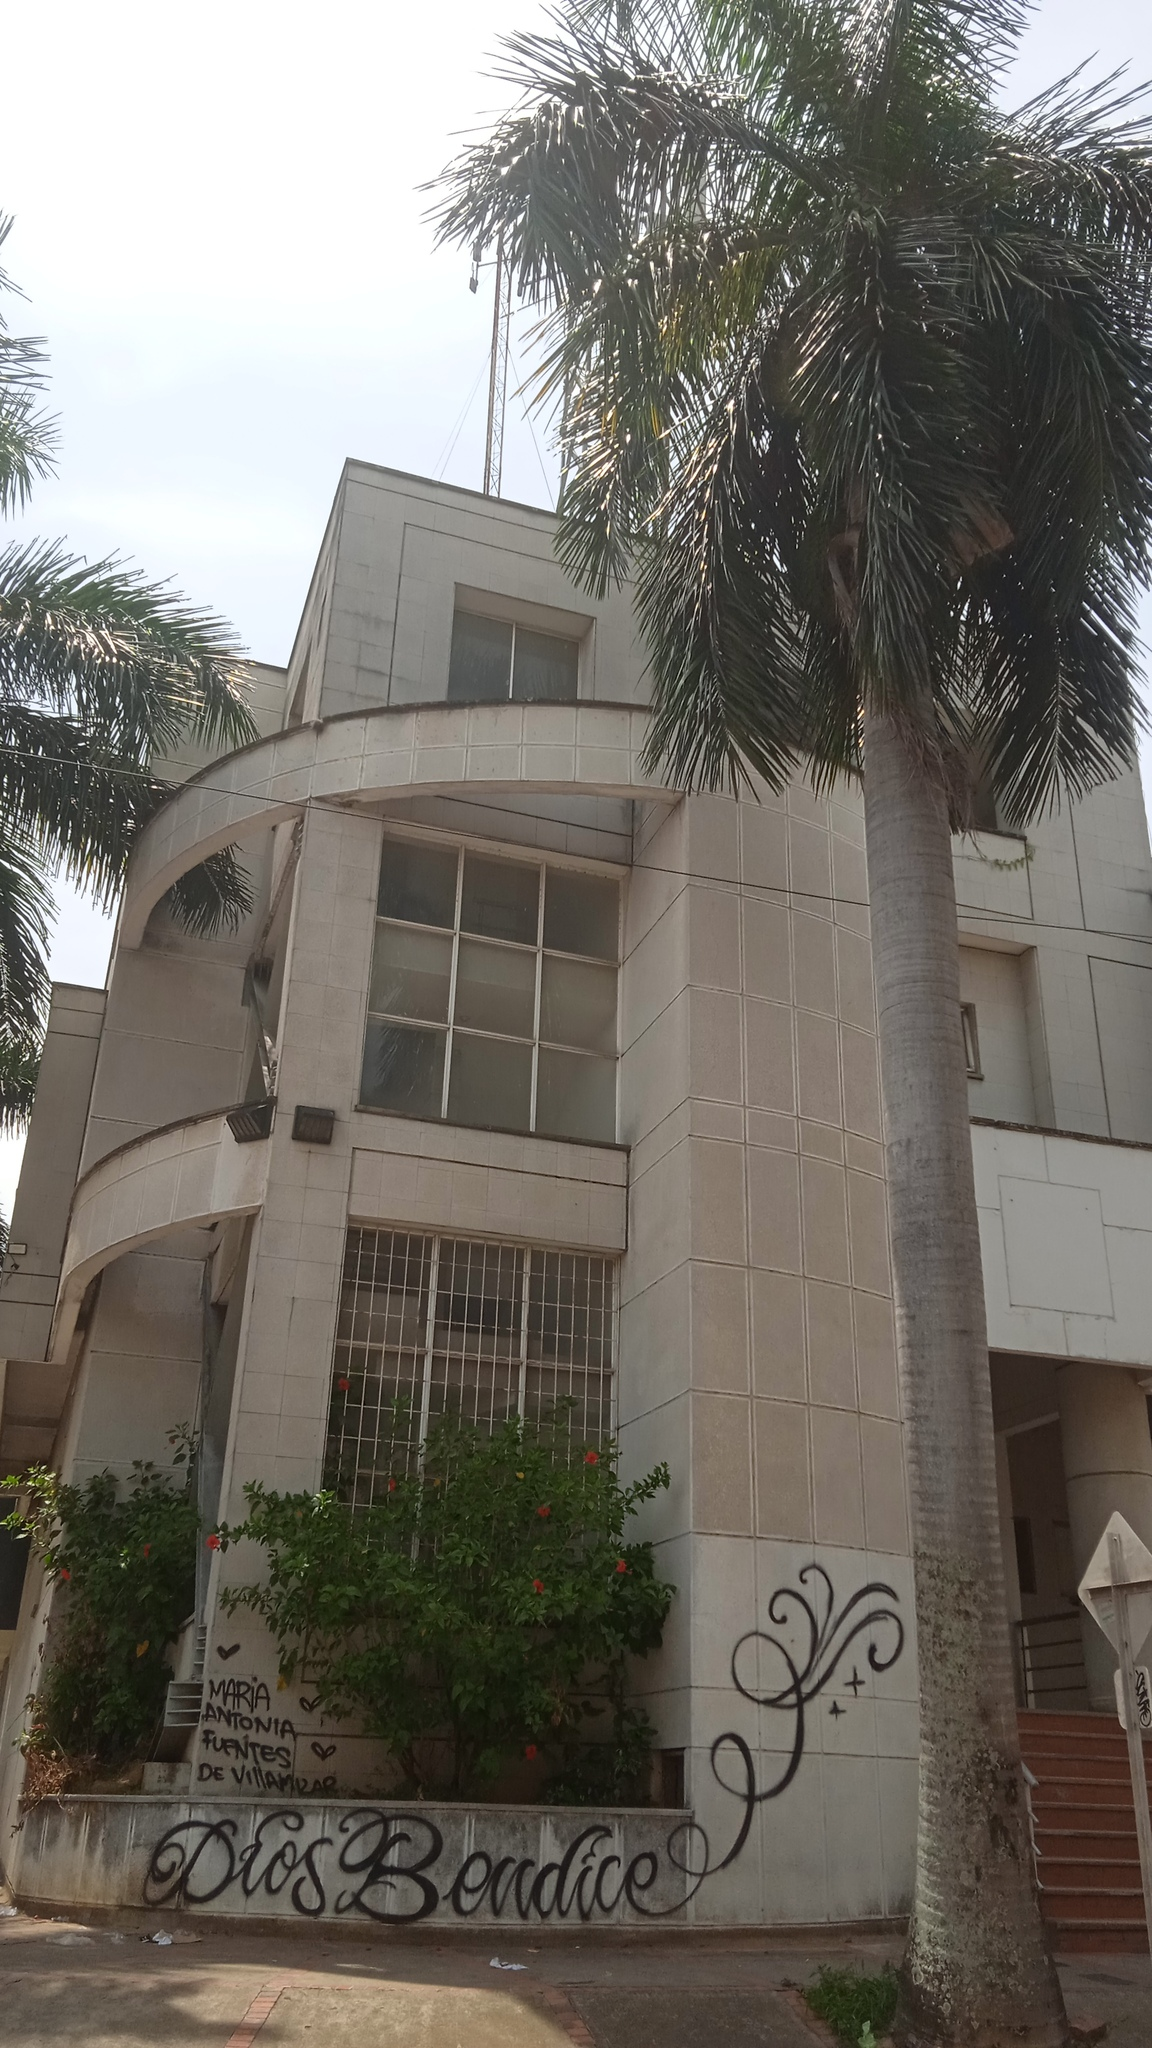
\includegraphics[width = 3 cm]{Imagenes/4} \\
	ENTORNO & FACHADA\\
	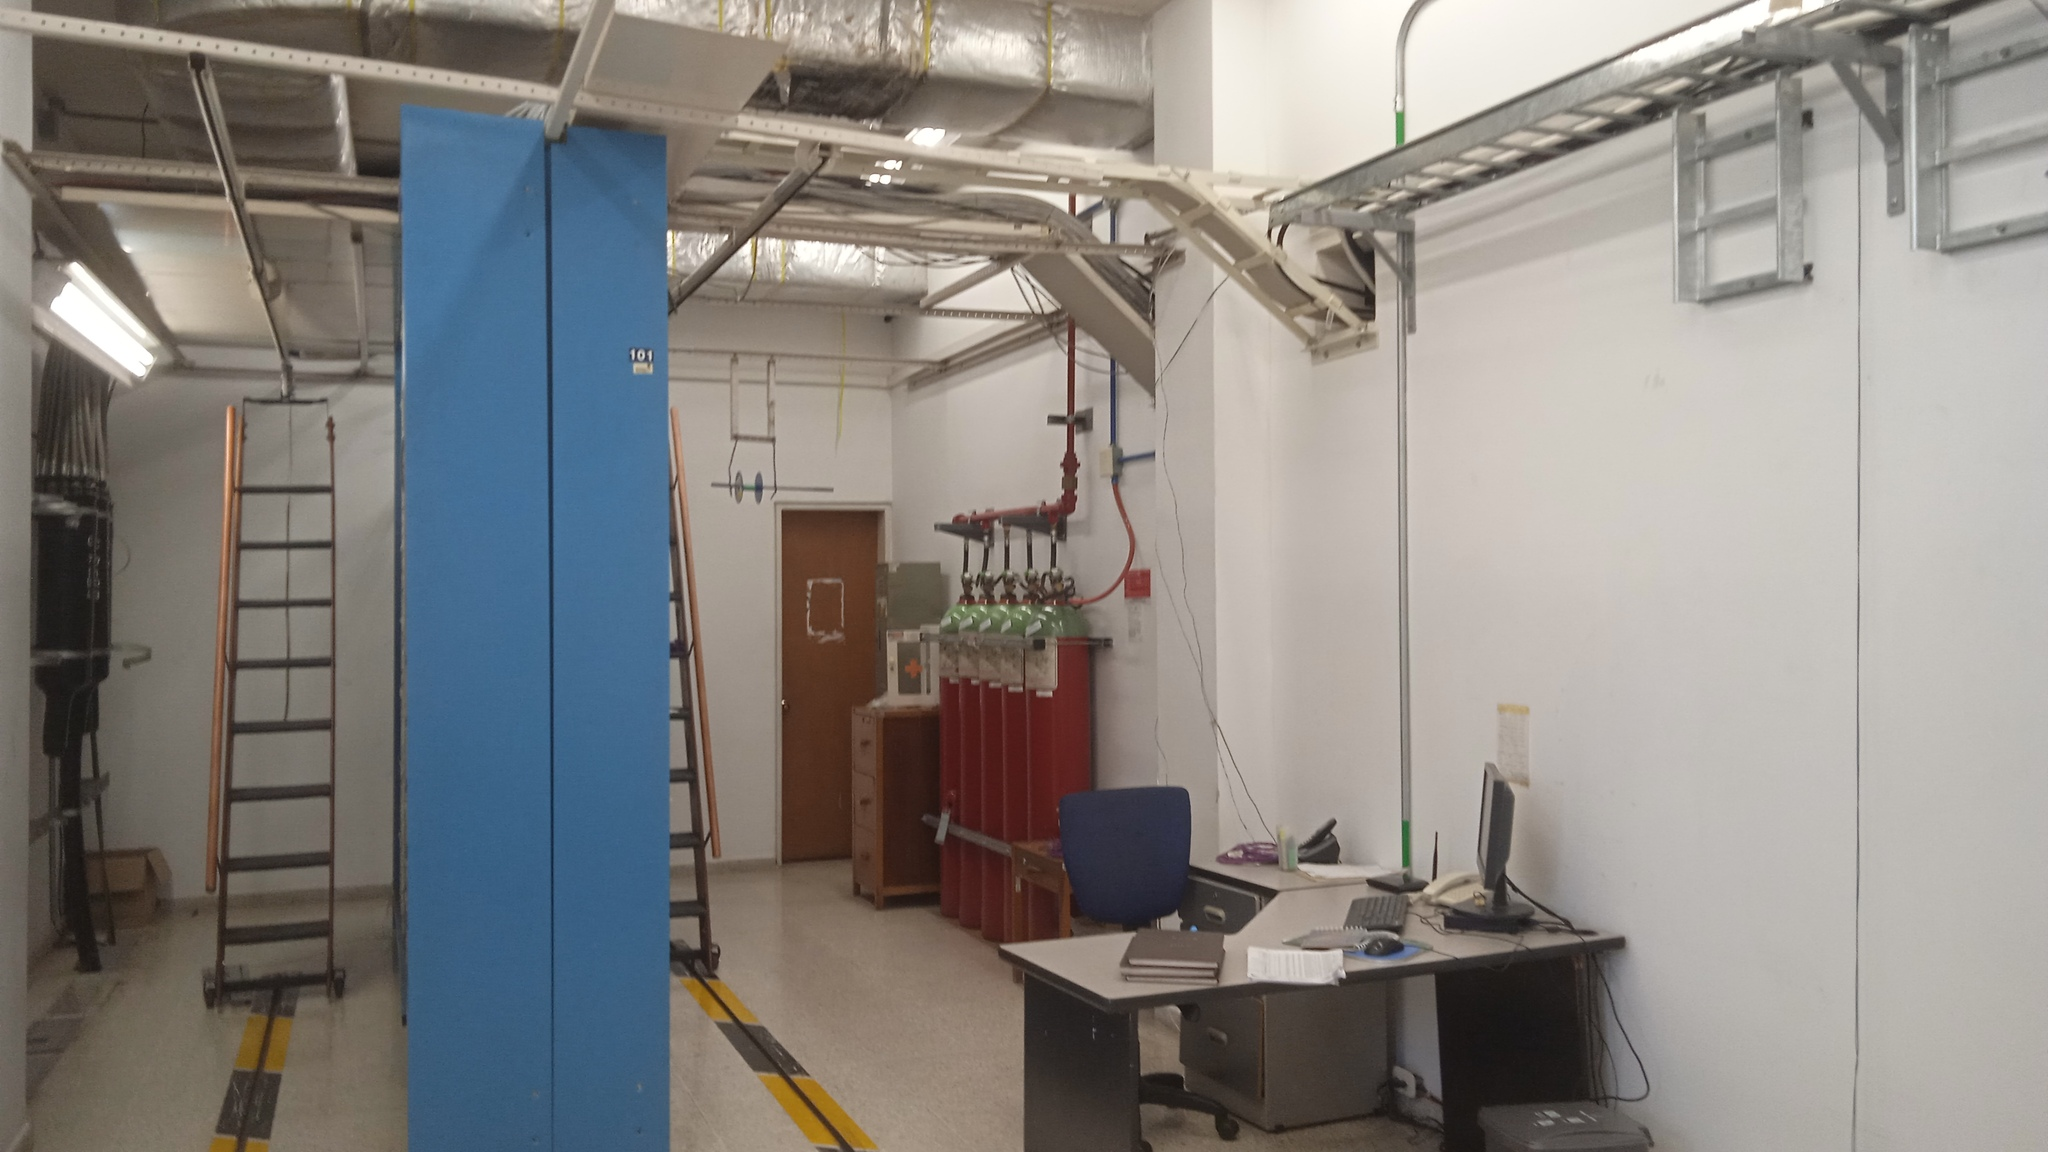
\includegraphics[width = 7 cm]{Imagenes/5} & 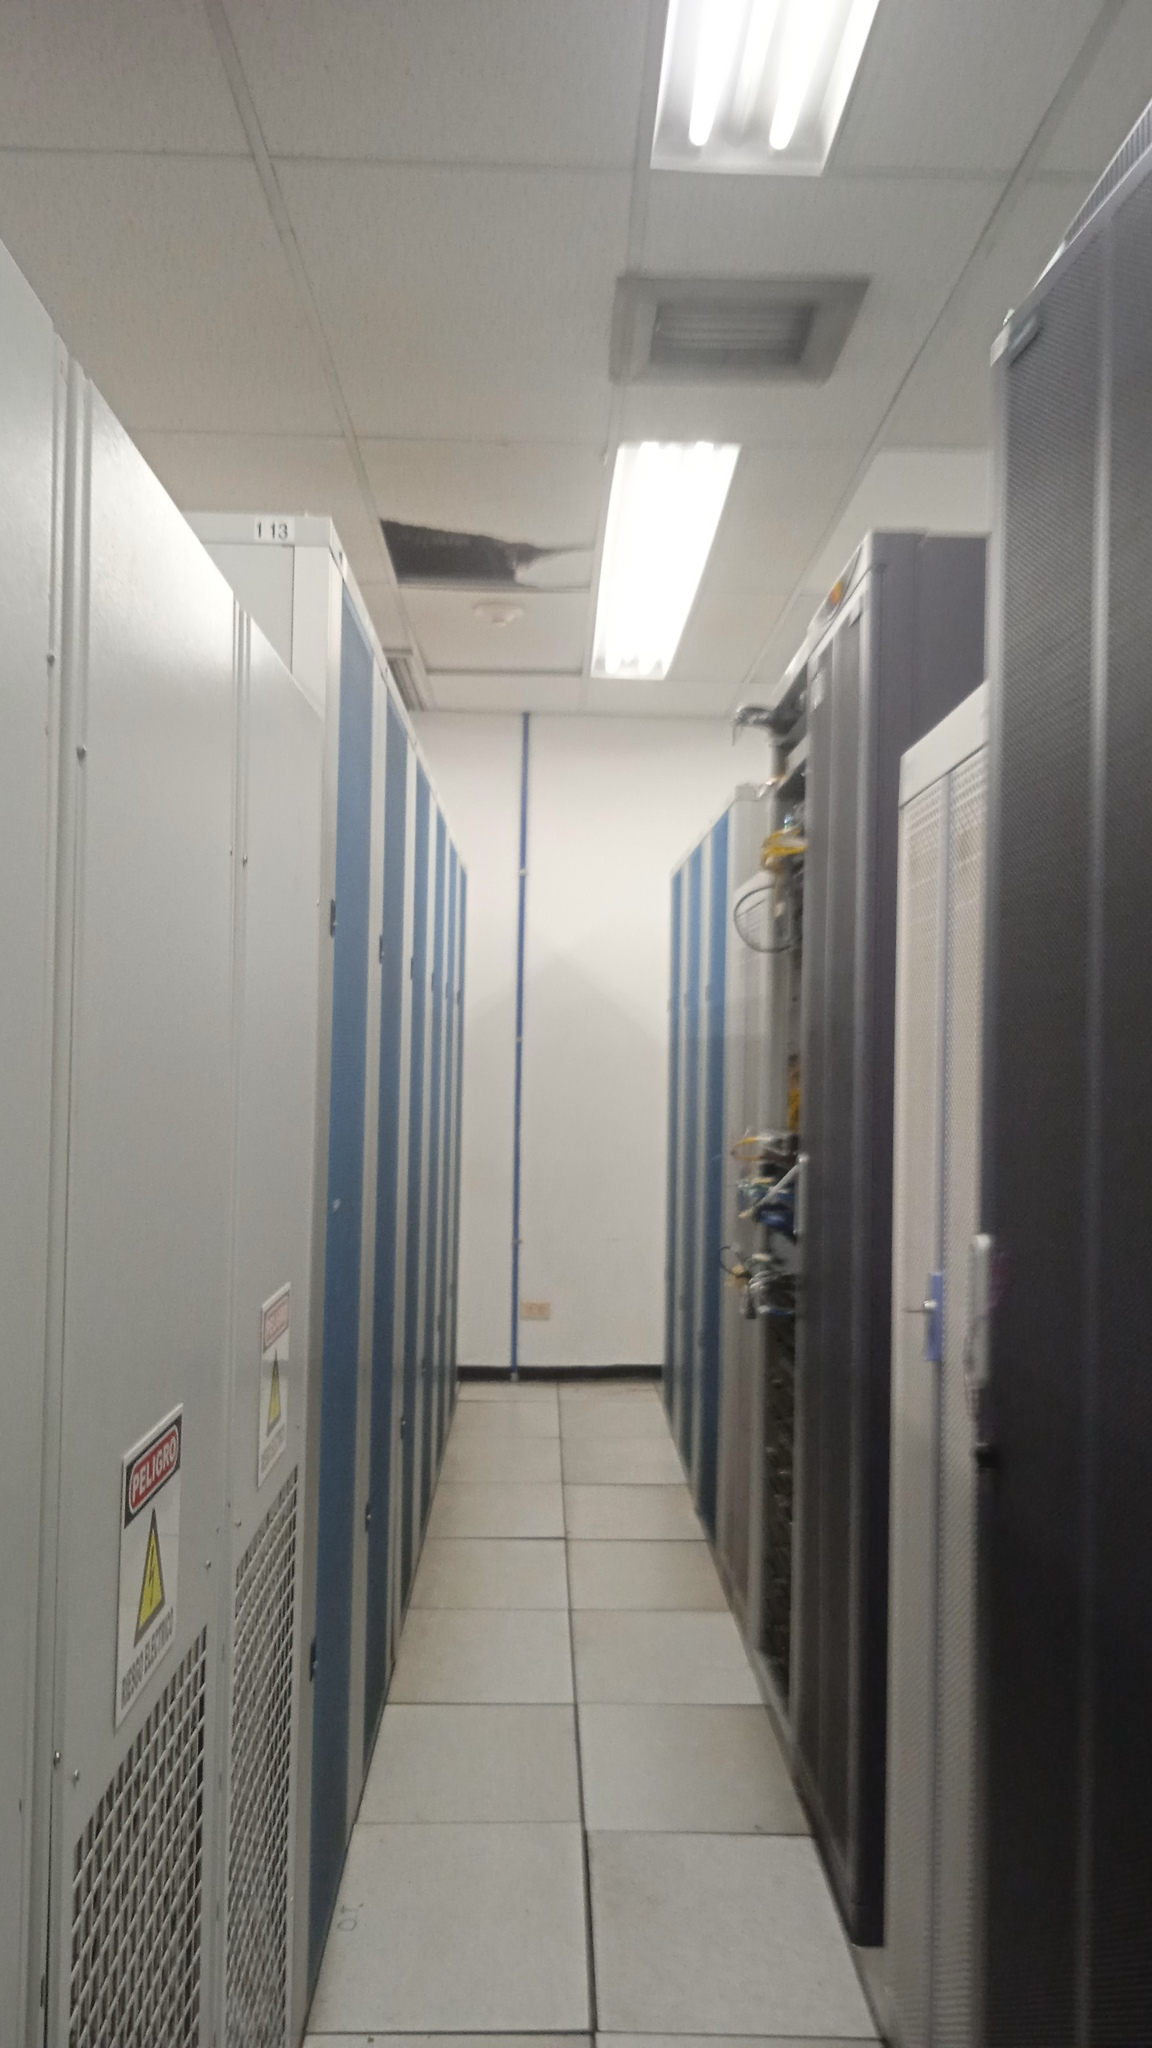
\includegraphics[width = 3 cm]{Imagenes/6} \\
	ÁREA TÉCNICA  & ÁREA TÉCNICA   \\
%	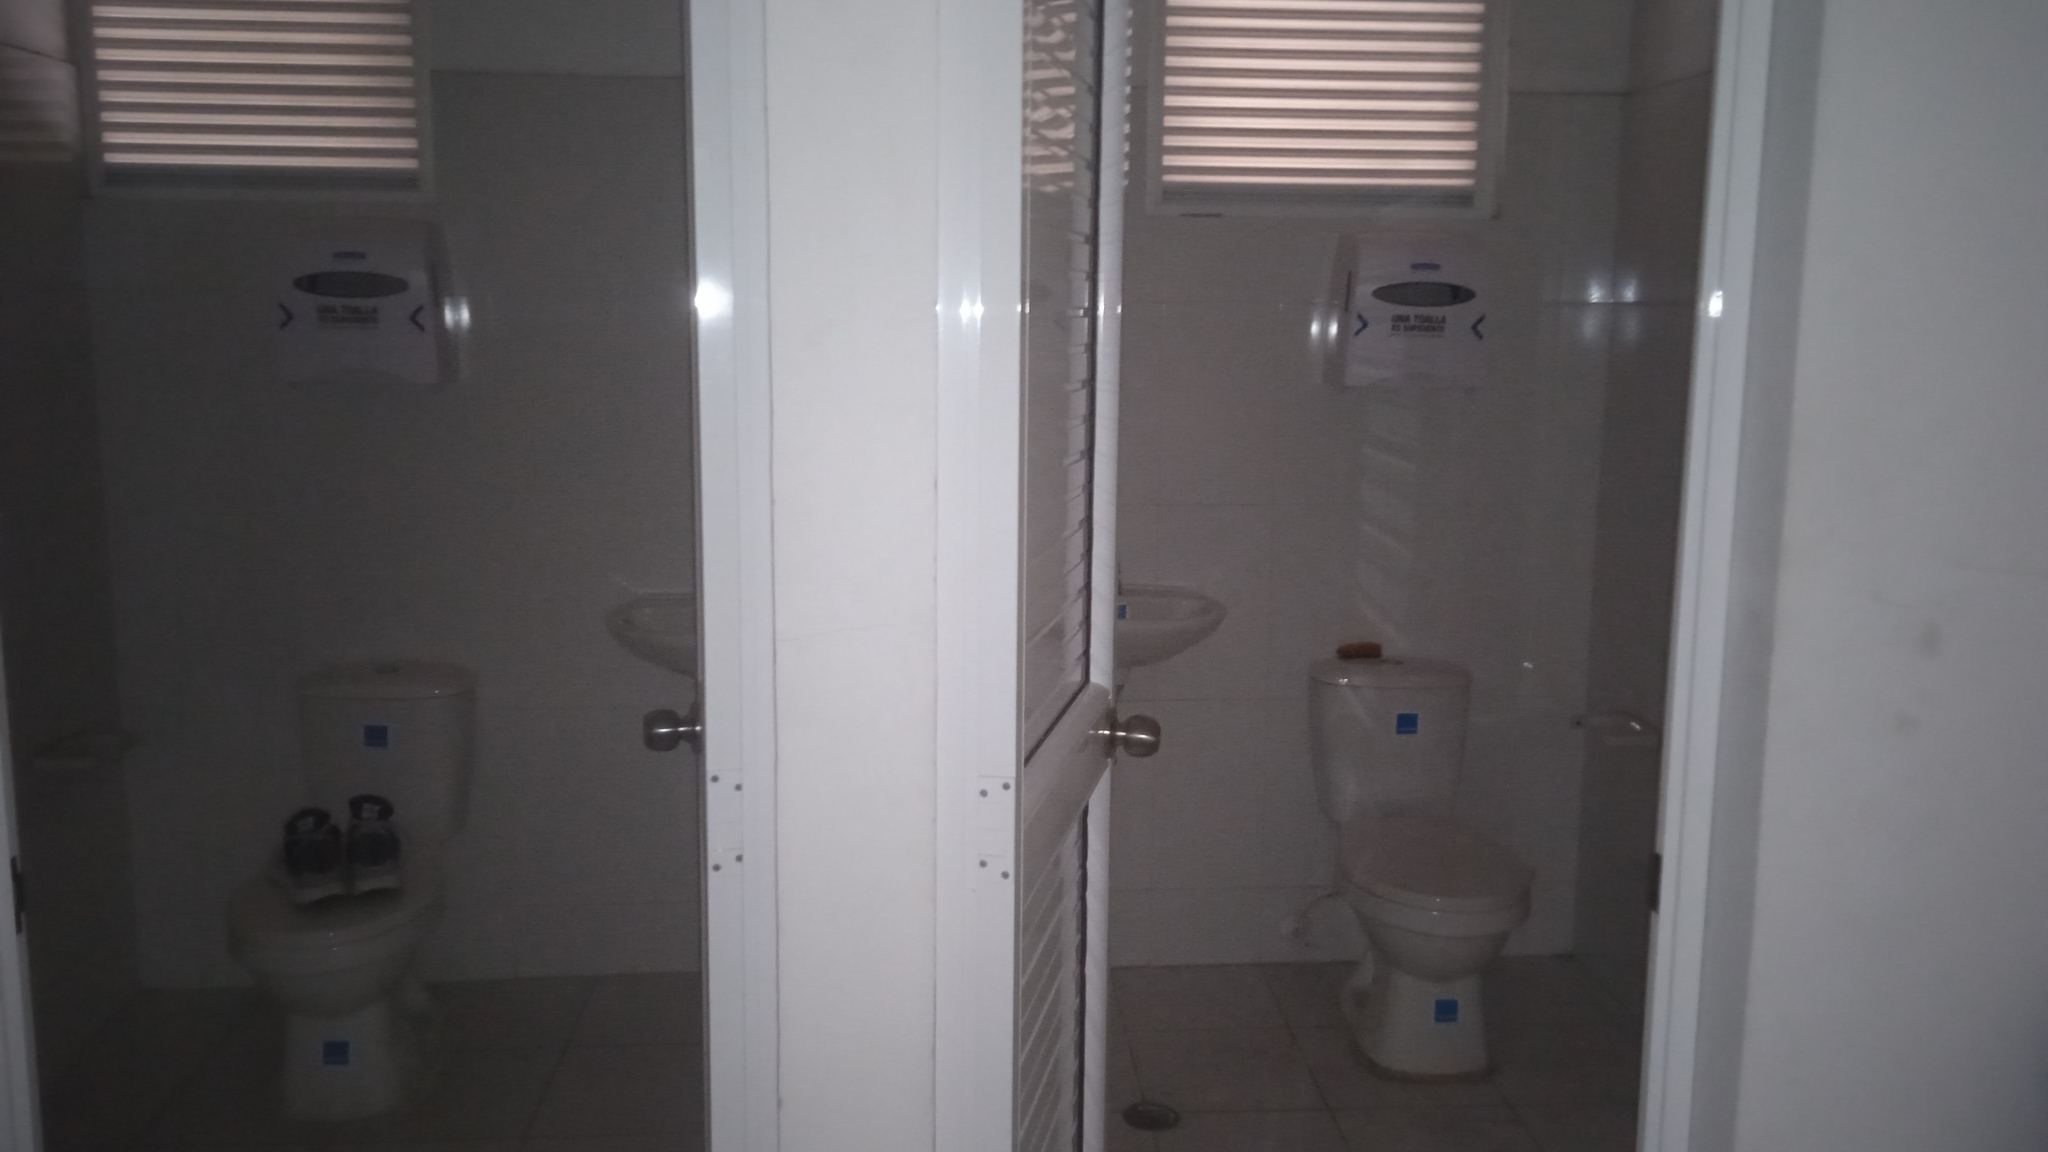
\includegraphics[width = 4 cm]{Imagenes/7} & 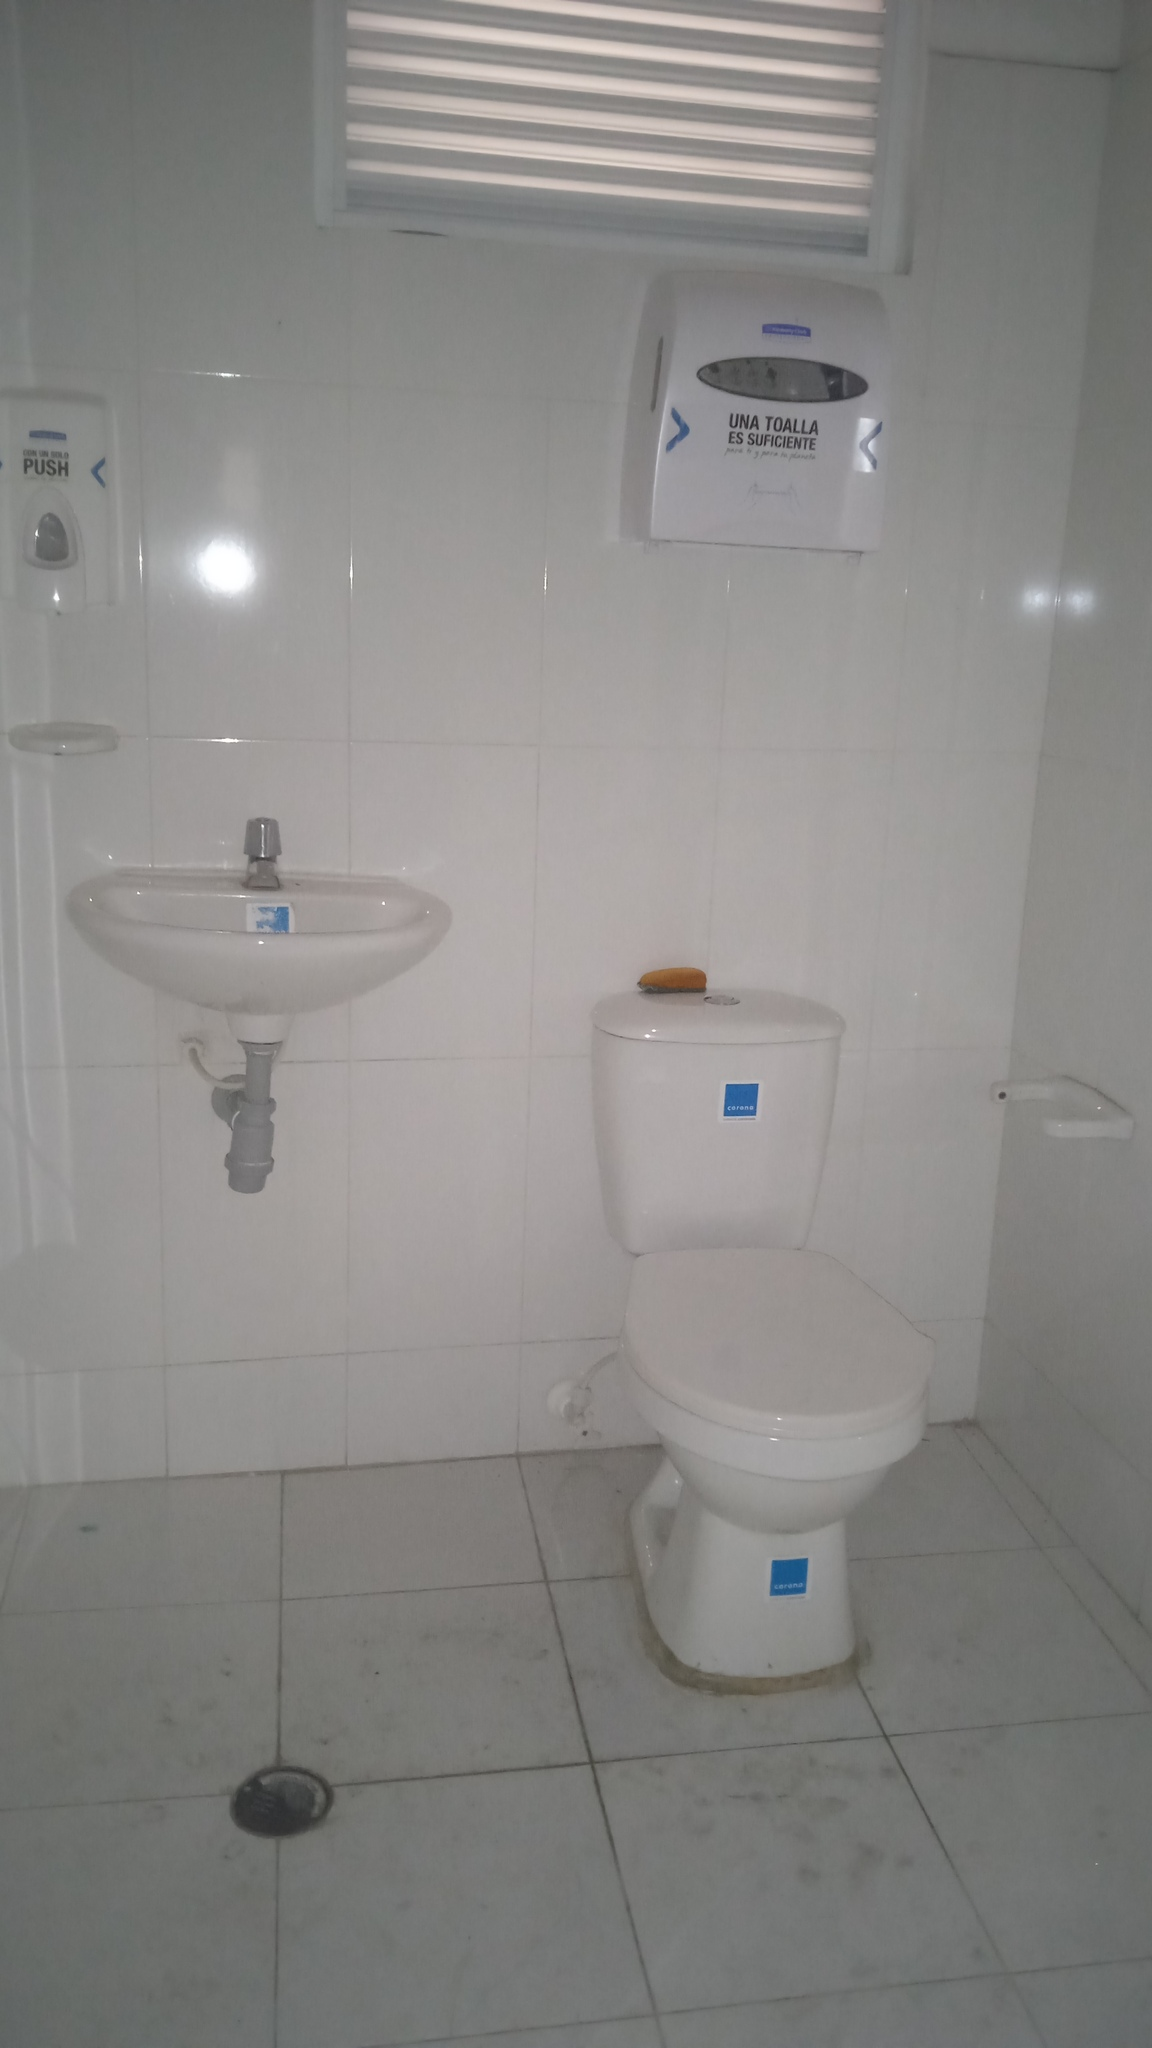
\includegraphics[width = 4 cm]{Imagenes/8} \\
%	COCINA  & ZONAS DE CIRCULACIÓN \\

	
\end{tabular} 

\begin{tabular}{ c c }
	
	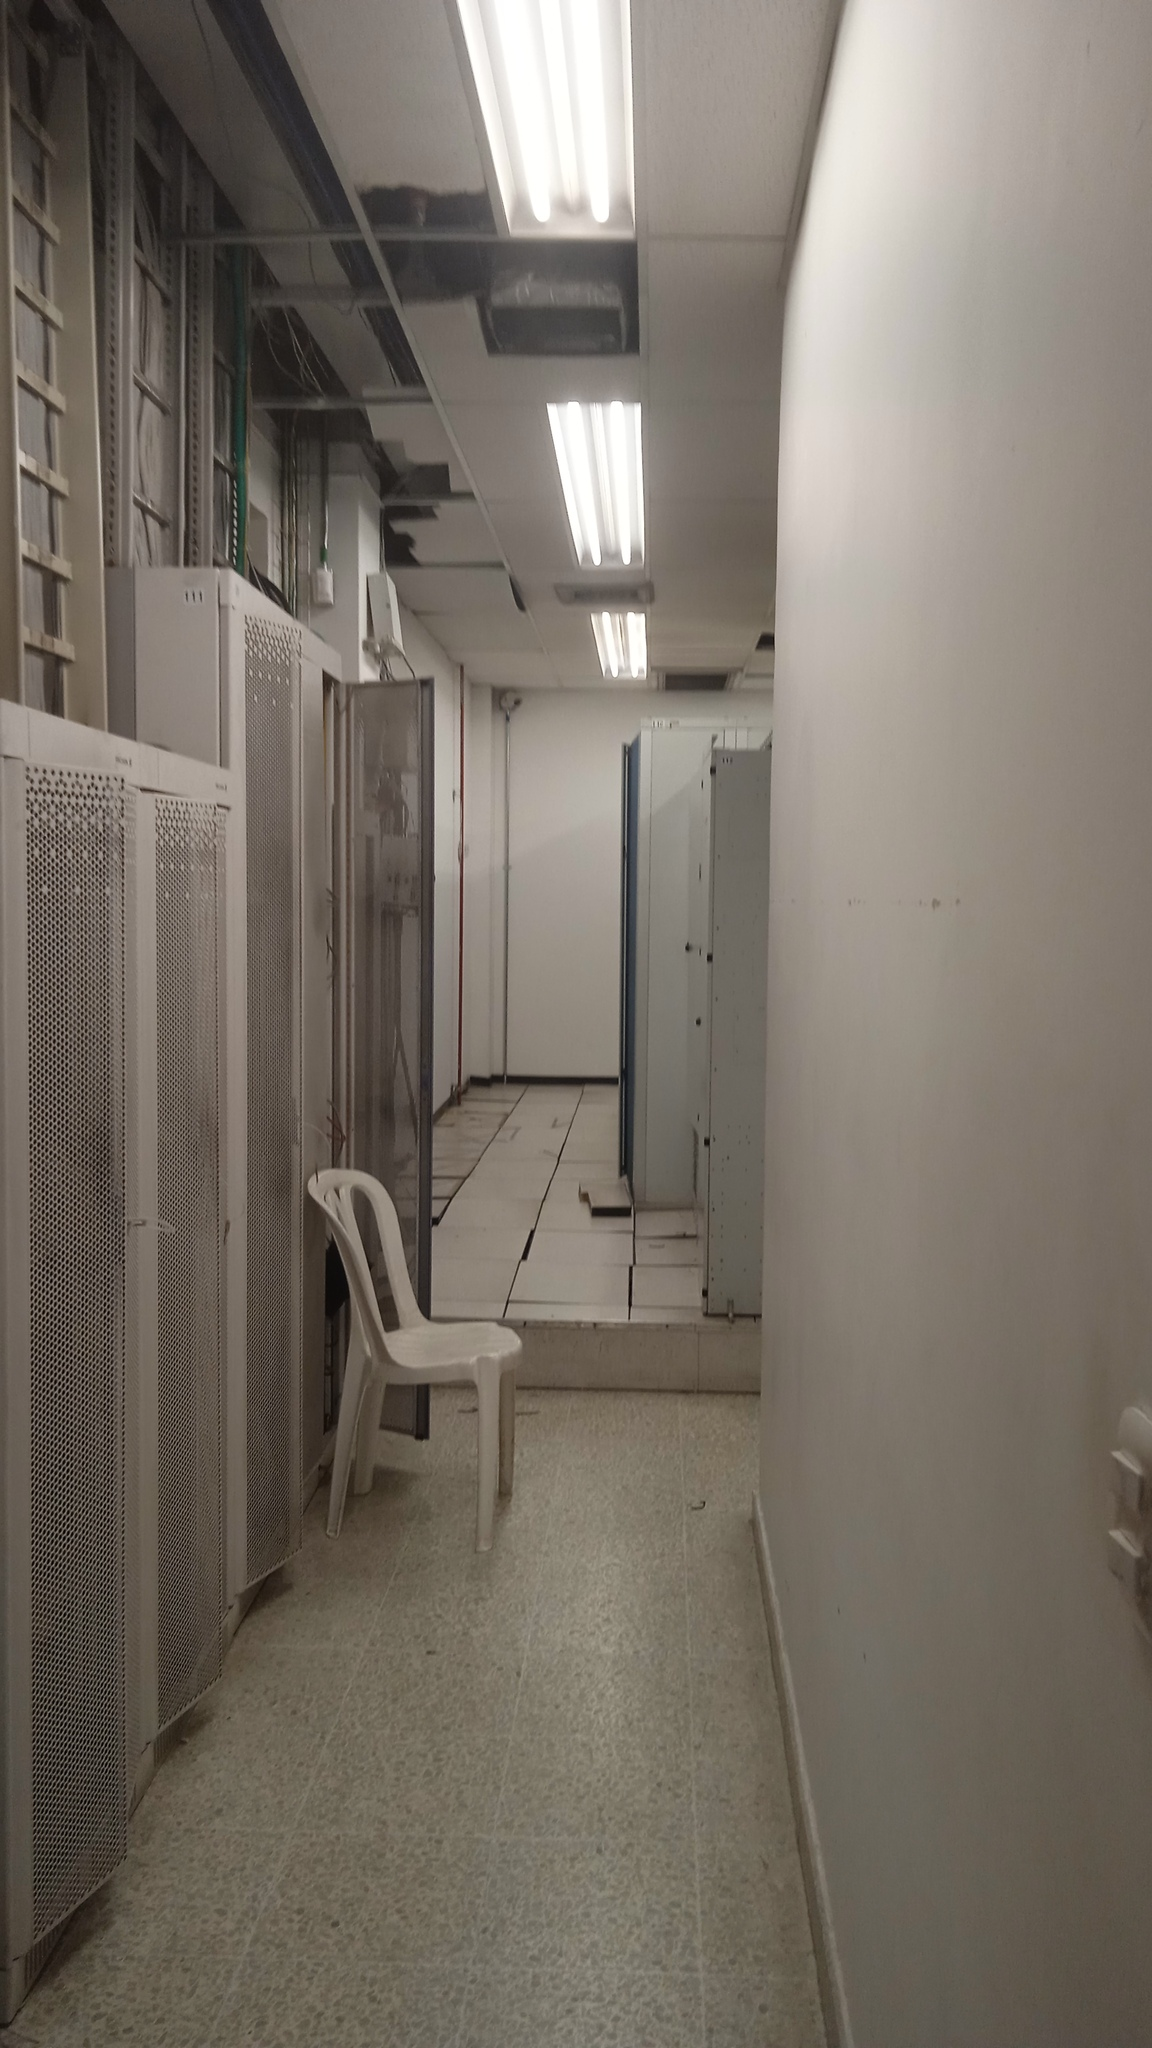
\includegraphics[width = 3 cm]{Imagenes/9} & 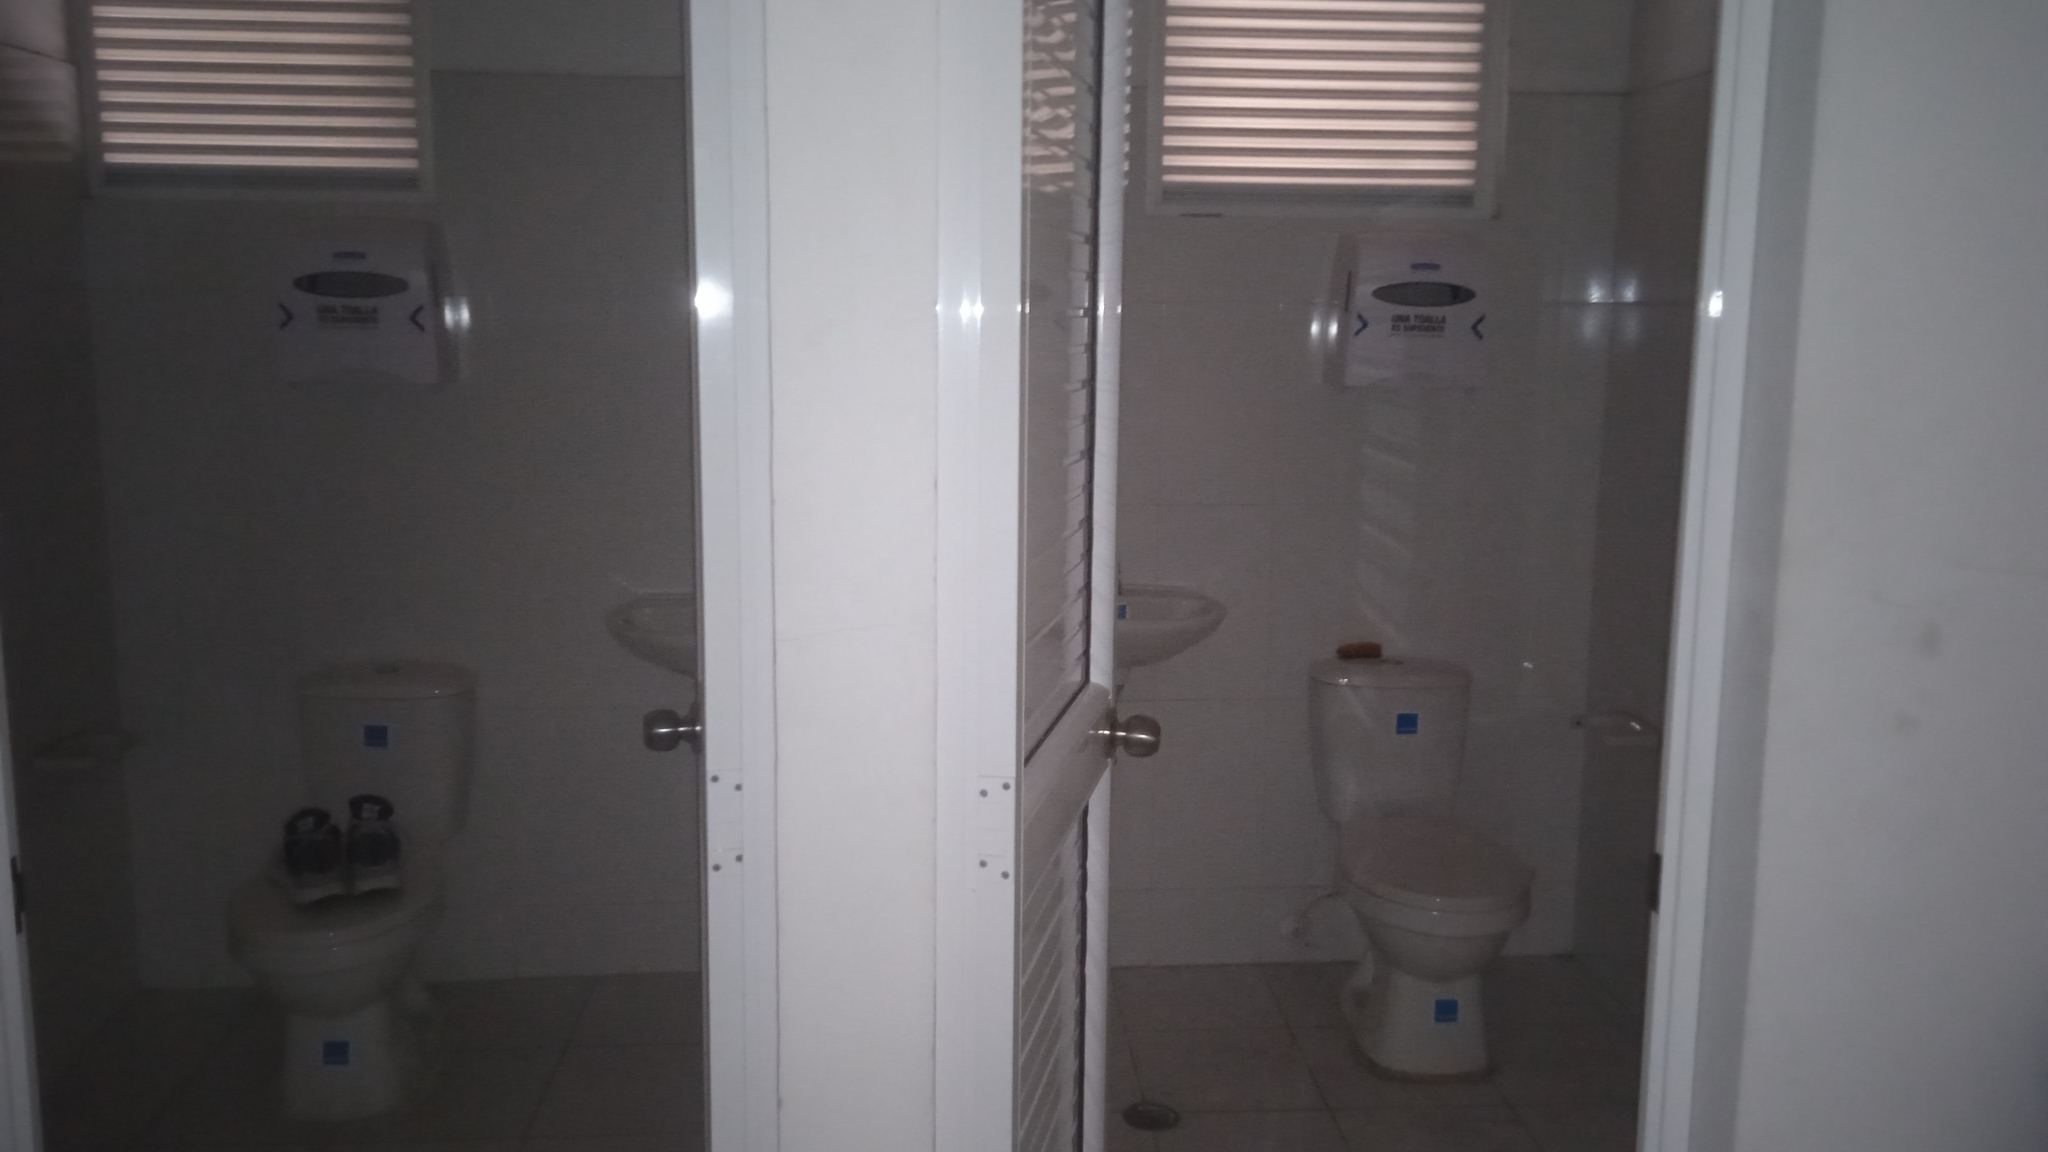
\includegraphics[width = 7 cm]{Imagenes/7} \\
	ÁREA TÉCNICA  & BAÑOS\\
	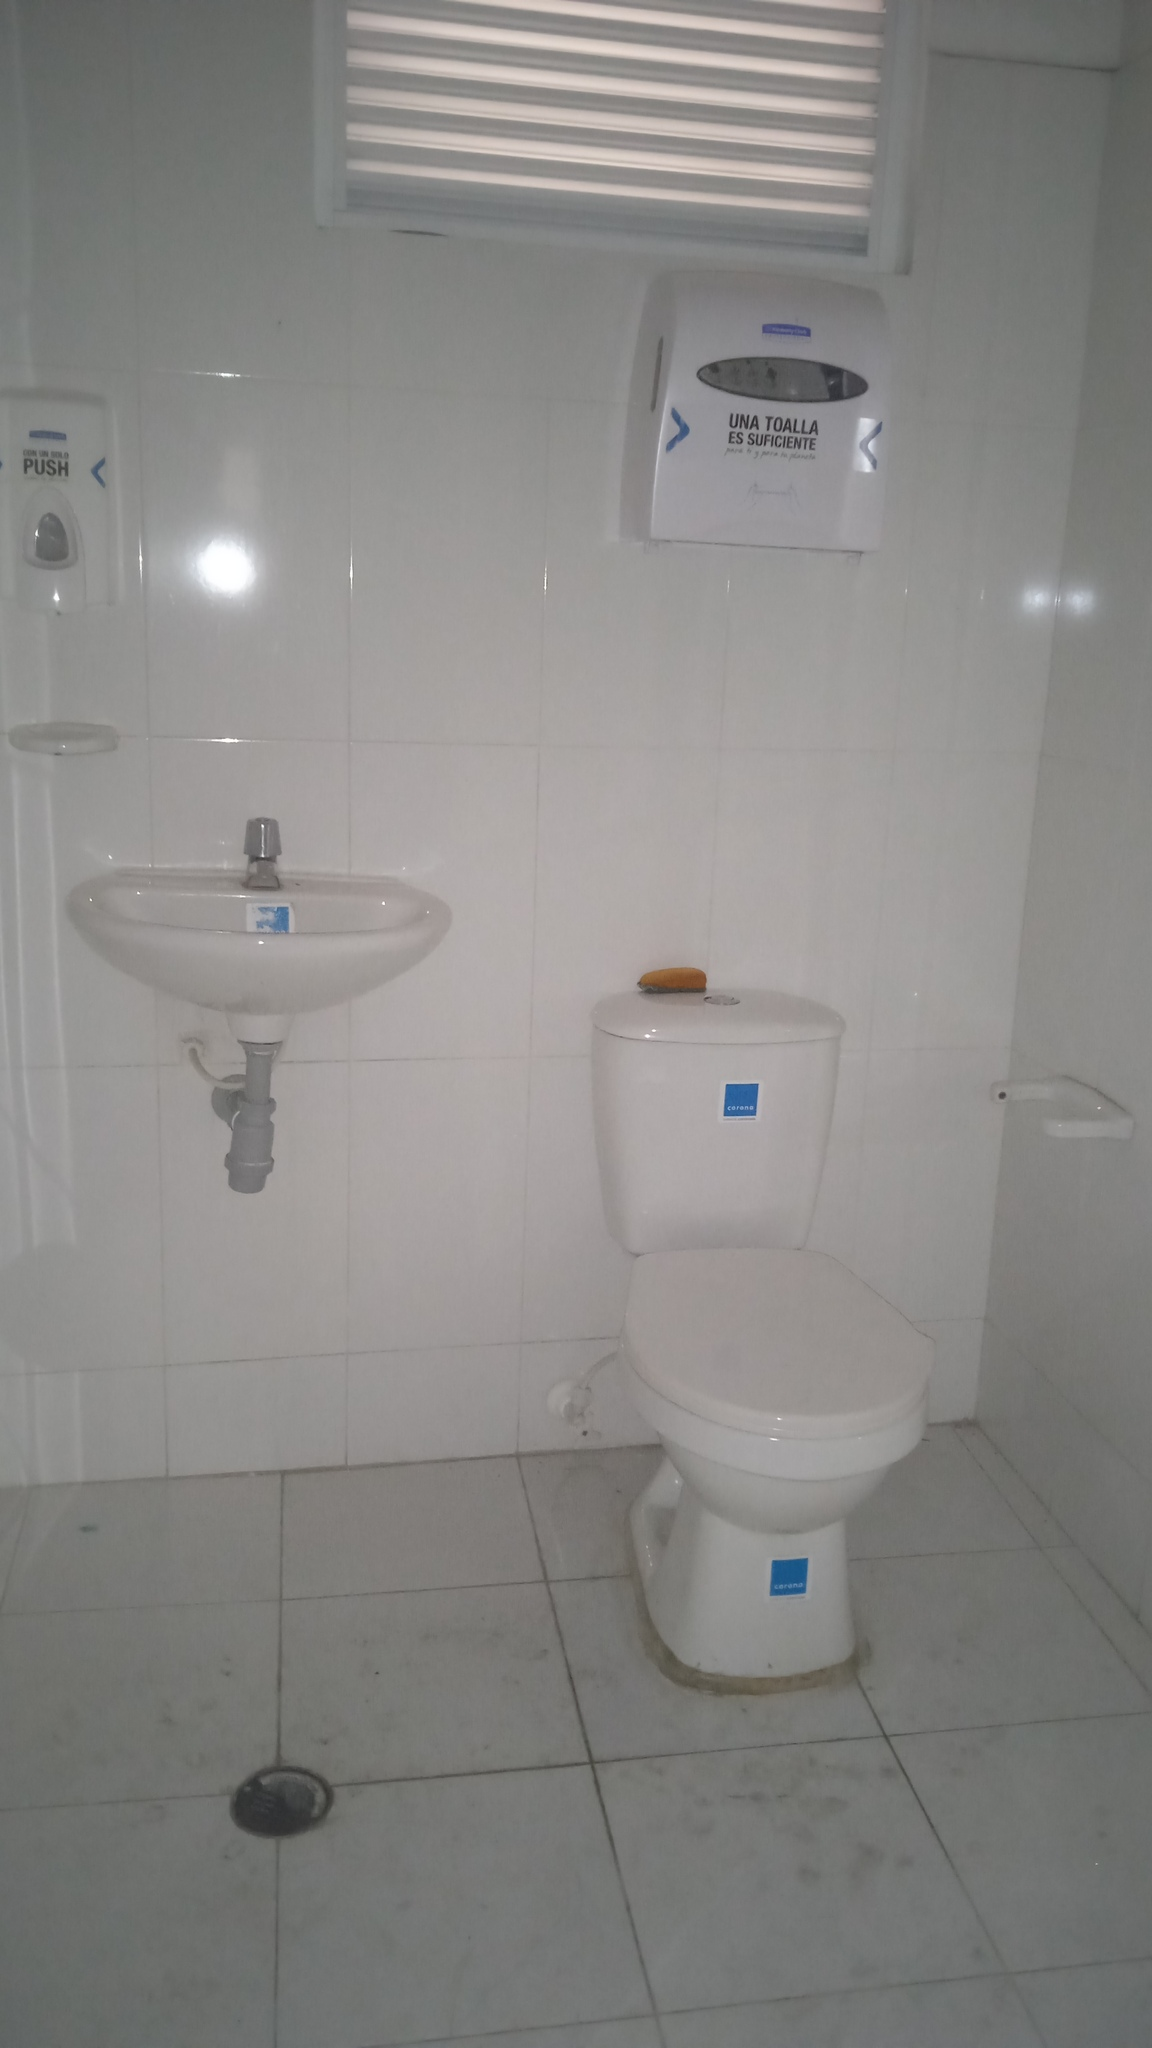
\includegraphics[width = 3 cm]{Imagenes/8} & 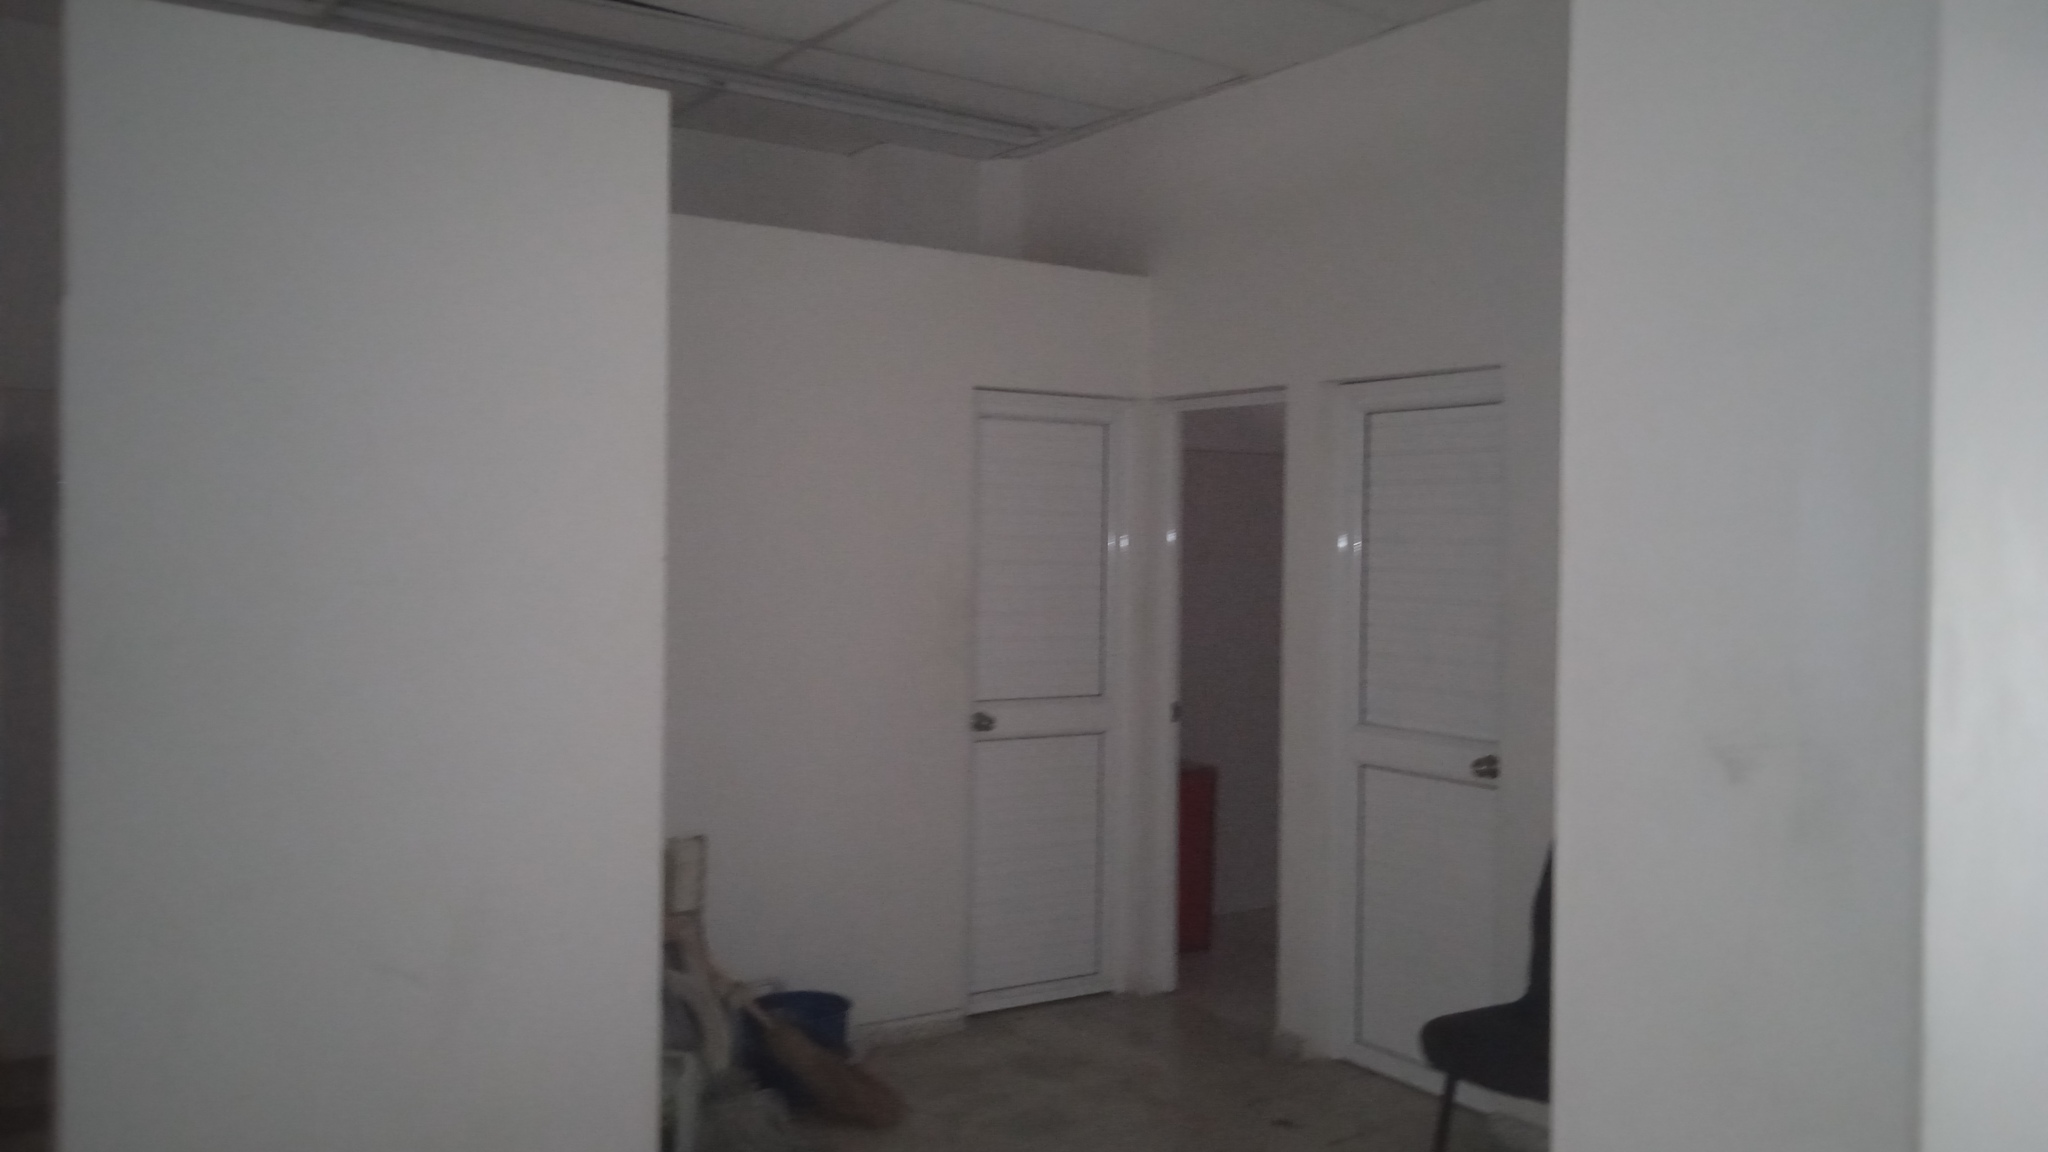
\includegraphics[width = 7 cm]{Imagenes/12} \\
	BAÑO & ÁREA OFICINA \\
	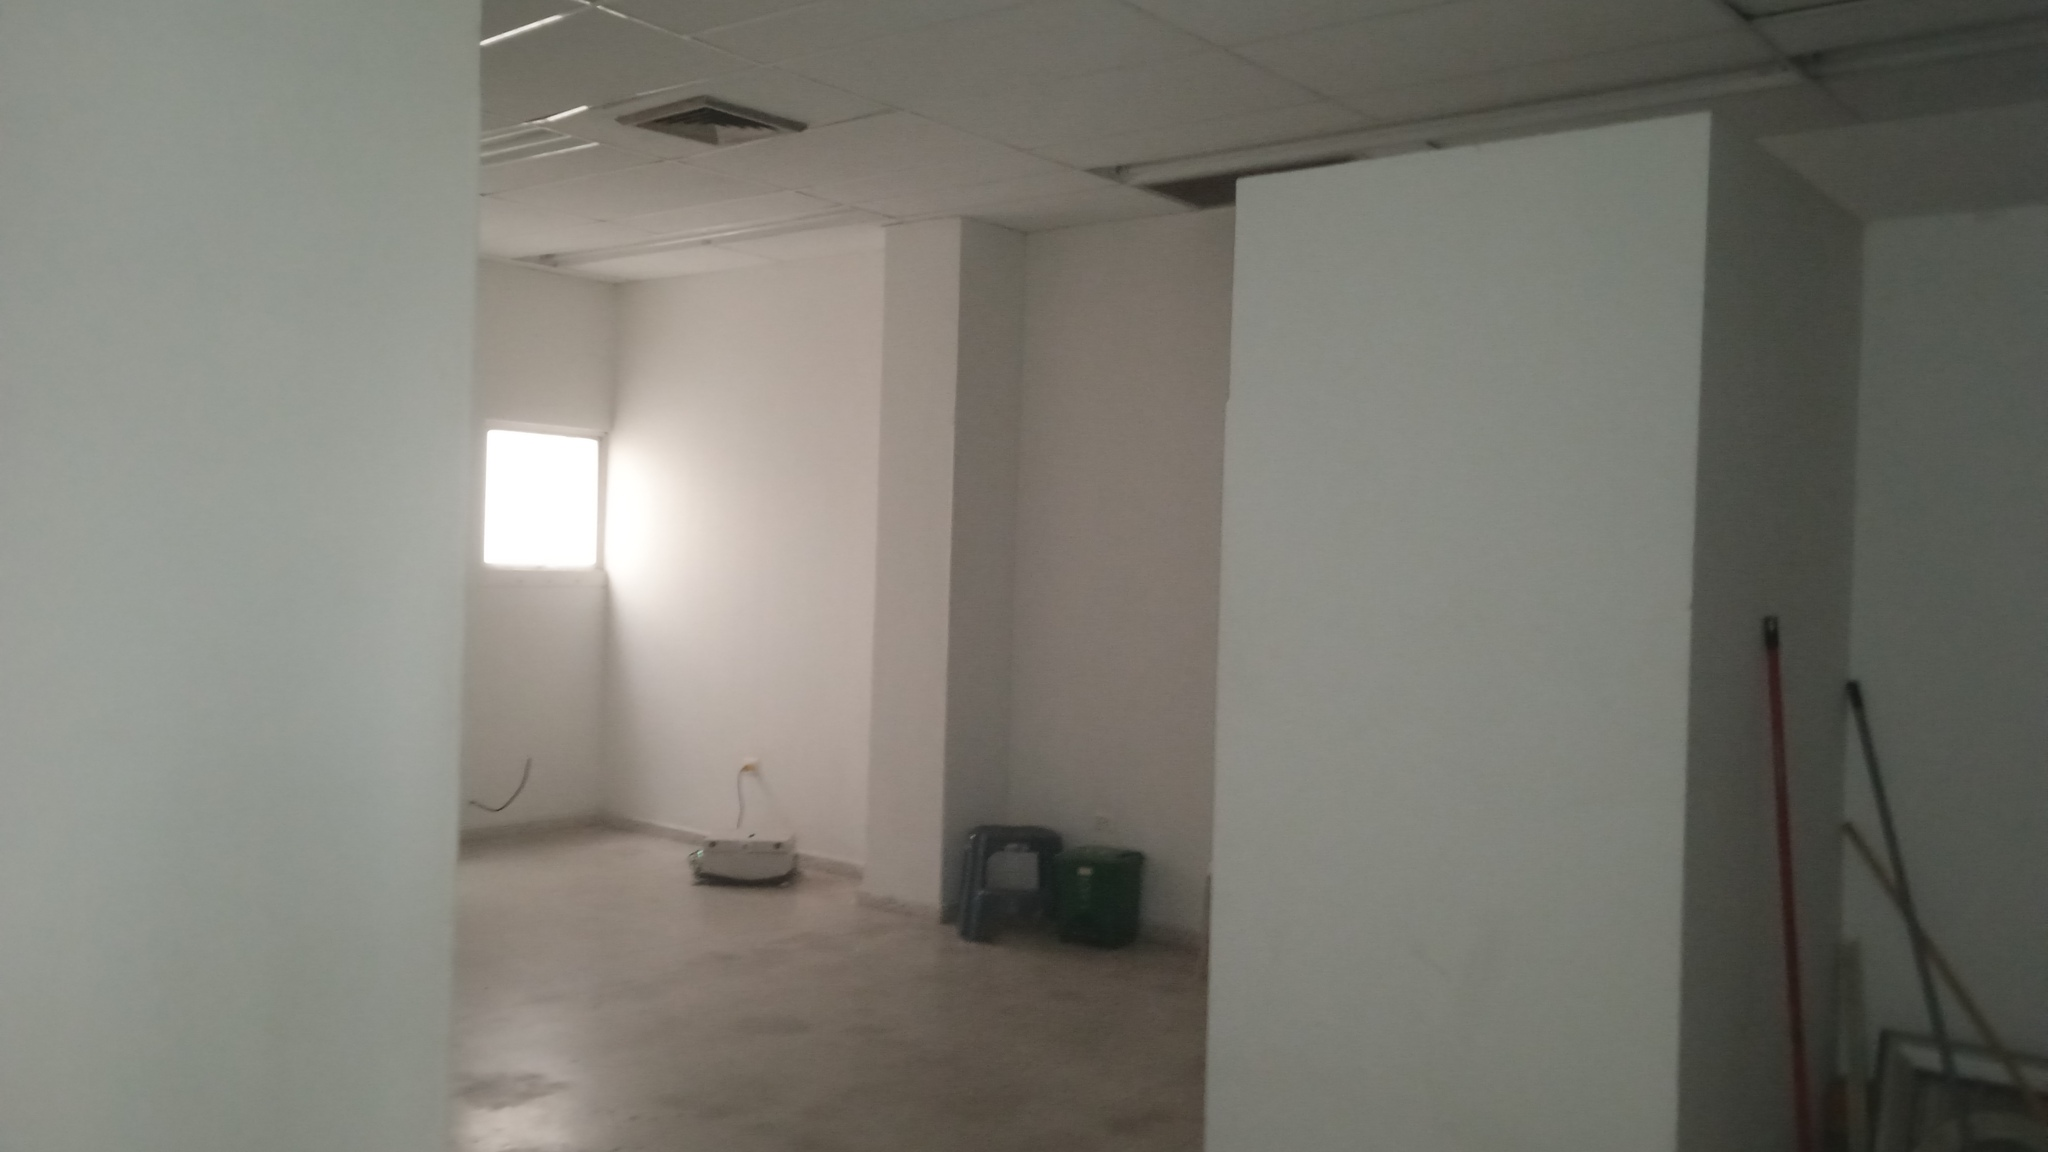
\includegraphics[width = 7 cm]{Imagenes/13} & \includegraphics[width = 7 cm]{Imagenes/14} \\
	ÁREA OFICINA & HALL\\
	\includegraphics[width = 7 cm]{Imagenes/15} & \includegraphics[width = 7 cm]{Imagenes/16} \\
	PISO 2  &  BAÑOS\\

	
\end{tabular} 

\begin{tabular}{ c c }
	
	\includegraphics[width = 3 cm]{Imagenes/17} & \includegraphics[width = 7 cm]{Imagenes/18} \\
    BAÑOS & ÁREA TÉCNICA \\
	\includegraphics[width = 7 cm]{Imagenes/19} & \includegraphics[width = 7 cm]{Imagenes/20} \\
	BALCON & HALL\\
	\includegraphics[width = 7 cm]{Imagenes/21} & \includegraphics[width = 7 cm]{Imagenes/22} \\
    ÁREA TÉCNICA & ÁREA TÉCNICA\\
	\includegraphics[width = 7 cm]{Imagenes/23} & \includegraphics[width = 7 cm]{Imagenes/24} \\
    PISO 3 & ÁREA TÉCNICA\\
%	\includegraphics[width = 7 cm]{Imagenes/29} & \includegraphics[width = 7 cm]{Imagenes/30} \\

	
\end{tabular} 

\begin{tabular}{ c c }
	
	\includegraphics[width = 7 cm]{Imagenes/25} & \includegraphics[width = 7 cm]{Imagenes/26} \\
	ÁREA TÉCNICA & ÁREA OFICINAS\\
	\includegraphics[width = 7 cm]{Imagenes/27} & \includegraphics[width = 7 cm]{Imagenes/28} \\
	DETALLE PISO & ÁREA OFICINAS\\
		\includegraphics[width = 7 cm]{Imagenes/29} & \includegraphics[width = 7 cm]{Imagenes/30} \\
ÁREA OFICINAS & ÁREA OFICINAS\\
	\includegraphics[width = 7 cm]{Imagenes/31} & \includegraphics[width = 7 cm]{Imagenes/32} \\
DETALLE PISO & ACCESO TERRAZA\\
	\includegraphics[width = 7 cm]{Imagenes/33} & \includegraphics[width = 7 cm]{Imagenes/34} \\
ANTENA & TERRAZA\\
\end{tabular}

\begin{tabular}{ c c }
	
	
\includegraphics[width = 7 cm]{Imagenes/35} & \includegraphics[width = 7 cm]{Imagenes/36} \\
	TERRAZA & TERRAZA\\
	\includegraphics[width = 7 cm]{Imagenes/37} & \includegraphics[width = 3 cm]{Imagenes/38} \\
	TERRAZA & ANTENA\\
		\includegraphics[width = 7 cm]{Imagenes/39} & \includegraphics[width = 7 cm]{Imagenes/40} \\
	SOTANO & SOTANO \\
	\includegraphics[width = 7 cm]{Imagenes/44} & \includegraphics[width = 7 cm]{Imagenes/42} \\
	PLANTA ELÉCTRICA & PLANTA ELÉCTRICA\\
	
%	
\end{tabular}
%

%
%\begin{tabular}{ c c }
%	
%	\includegraphics[width = 3 cm]{Imagenes/49} & \includegraphics[width = 9 cm]{Imagenes/50} \\
%	Detalle piso 2 & Detalle piso 2\\
%	\includegraphics[width = 3 cm]{Imagenes/51} & \includegraphics[width = 3 cm]{Imagenes/52} \\
%	Detalle piso 2 & Detalle piso 2\\
%	\includegraphics[width = 3 cm]{Imagenes/53} & \includegraphics[width = 3 cm]{Imagenes/54} \\
%	Detalle piso 2 & Detalle piso 2\\
%	
%\end{tabular}
%
%\begin{tabular}{ c c }
%	DETALLE LOTE
%	\includegraphics[width = 3 cm]{Imagenes/55} & \includegraphics[width = 3 cm]{Imagenes/56} \\
%	Detalle piso 2 & Detalle piso 2\\
%	\includegraphics[width = 3 cm]{Imagenes/57} & \includegraphics[width = 3 cm]{Imagenes/58} \\
%	Detalle piso 2 & Detalle piso 2\\
%	\includegraphics[width = 3 cm]{Imagenes/59} & \includegraphics[width = 3 cm]{Imagenes/60} \\
%	Escaleras acceso piso 3 & Detalle piso 3\\
%	
%\end{tabular}
%
%\begin{tabular}{ c c }
%	
%	\includegraphics[width = 3 cm]{Imagenes/61} & \includegraphics[width = 3 cm]{Imagenes/62} \\
%	Detalle piso 3 & Detalle piso 3\\
%	\includegraphics[width = 3 cm]{Imagenes/63} & \includegraphics[width = 3 cm]{Imagenes/64} \\
%	Detalle piso 3 & Detalle piso 3\\
%	\includegraphics[width = 3 cm]{Imagenes/65} & \includegraphics[width = 3 cm]{Imagenes/66} \\
%	Cuarto técnico & Cuarto técnico\\
%	
%\end{tabular}
%
%\begin{tabular}{ c c }
%	
%	\includegraphics[width = 3 cm]{Imagenes/67} & \includegraphics[width = 3 cm]{Imagenes/68} \\
%	Zona de oficinas & Detalle estructura\\
%	\includegraphics[width = 3 cm]{Imagenes/69} & \includegraphics[width = 3 cm]{Imagenes/70} \\
%	Piso 2 & Zona de oficinas\\
%	\includegraphics[width = 3 cm]{Imagenes/71} & \includegraphics[width = 3 cm]{Imagenes/72} \\
%	Detalle piso 3 & Detalle piso 3\\
%	
%\end{tabular}
%
%\begin{tabular}{ c c }
%	
%	\includegraphics[width = 3 cm]{Imagenes/73} & \includegraphics[width = 3 cm]{Imagenes/74} \\
%	Detalle piso 3 & Detalle estructura\\
%	\includegraphics[width = 3 cm]{Imagenes/75} & \includegraphics[width = 3 cm]{Imagenes/76} \\
%	Piso 2 & Zona de Escaleras acceso piso 4\\
%	\includegraphics[width = 3 cm]{Imagenes/77} & \includegraphics[width = 3 cm]{Imagenes/78} \\
%	Detalle piso 4 & Detalle piso 4\\
%	
%\end{tabular}
%
%\begin{tabular}{ c c }
%	
%	\includegraphics[width = 3 cm]{Imagenes/79} & \includegraphics[width = 3 cm]{Imagenes/80} \\
%	Detalle piso 4 & Detalle piso 4\\
%	\includegraphics[width = 3 cm]{Imagenes/81} & \includegraphics[width = 3 cm]{Imagenes/82} \\
%	Detalle piso 4 &  Detalle piso 4\\
%	\includegraphics[width = 7 cm]{Imagenes/83} & \includegraphics[width = 7 cm]{Imagenes/84} \\
%	Detalle terraza & Detalle terraza\\
%	
%\end{tabular}
%
%\begin{tabular}{ c c }
%	
%	\includegraphics[width = 3 cm]{Imagenes/85} & \includegraphics[width = 3 cm]{Imagenes/86} \\
%	Escaleras acceso terraza & Detalle terraza\\
%	\includegraphics[width = 3 cm]{Imagenes/87} & \includegraphics[width = 3 cm]{Imagenes/88} \\
%	Detalle terraza & Detalle terraza\\
%	\includegraphics[width = 3 cm]{Imagenes/89} & \includegraphics[width = 3 cm]{Imagenes/90} \\
%	Detalle terraza & Detalle terraza\\
%	
%\end{tabular}

%subsubsection*{Plano de localización}
%
%\includegraphics[width = 12 cm]{Imagenes/ubicacion.png}
%
%Indentificacion de subcontratistas y personal de apoyo. 

\end{document}
